\documentclass{article}

% if you need to pass options to natbib, use, e.g.:
%     \PassOptionsToPackage{numbers, compress}{natbib}
% before loading neurips_2020

% ready for submission
 \usepackage{neurips_2020}

% to compile a preprint version, e.g., for submission to arXiv, add add the
% [preprint] option:
%     \usepackage[preprint]{neurips_2020}

% to compile a camera-ready version, add the [final] option, e.g.:
%    \usepackage[final]{neurips_2020}

% to avoid loading the natbib package, add option nonatbib:
%     \usepackage[nonatbib]{neurips_2020}

\usepackage[utf8]{inputenc} % allow utf-8 input
\usepackage[T1]{fontenc}    % use 8-bit T1 fonts
\usepackage{hyperref}       % hyperlinks
\usepackage{url}            % simple URL typesetting
\usepackage{booktabs}       % professional-quality tables
\usepackage{amsfonts}       % blackboard math symbols
\usepackage{nicefrac}       % compact symbols for 1/2, etc.
\usepackage{microtype}      % microtypography

%Image-related packages
\usepackage{graphicx}
\usepackage{enumitem}
\bibliographystyle{unsrt}
\usepackage{algorithm} 
\usepackage{algpseudocode} 
\usepackage{subcaption}

\title{Supplementary Material of Spatio-Temporal Domain Adaptation for Gait Based User Recognition from Radar Data}

\author{
  Kalvik Jakkala \\
  Department of Computer Science\\
  University of North Carolina at Charlotte\\
  Charlotte, NC 28223 \\
  \texttt{kjakkala@uncc.edu} \\
  \And
  Chen Chen \\
  Department of Computer Science\\
  University of North Carolina at Charlotte\\
  Charlotte, NC 28223 \\
  \texttt{chen.chen@uncc.edu} \\
  \And
  Minwoo Lee \\
  Department of Computer Science\\
  University of North Carolina at Charlotte\\
  Charlotte, NC 28223 \\
  \texttt{minwoo.lee@uncc.edu} \\
  \And
  Arupjyoti    Bhuyan \\
  Idaho National Laboratory \\
  Idaho Falls, ID 83401 \\
  \texttt{arupjyoti.bhuyan@inl.gov} \\
  \And
  Zhi Sun \\
  Department of Electrical Engineering \\
  University at Buffalo    \\
  Buffalo, NY 14260 \\
  \texttt{zhisun@buffalo.edu} \\
  \And
  Pu Wang \\
  Department of Computer Science\\
  University of North Carolina at Charlotte\\
  Charlotte, NC 28223 \\
  \texttt{pu.wang@uncc.edu} \\
}

\begin{document}

\maketitle

\tableofcontents

\section{Dataset}
Our dataset was collected using a TI IWR1642 mmWave sensor \cite{iwr1642boost}. The radar chirp configuration used in \cite{janakaraj2019star} was utilized to collect data from 4 different locations. The primary location, which was used as the source domain, was a research lab with cubicles. Each of the ten subjects was asked to walk back and forth in the room with a radar pointed at them. The subject's path was pre-determined and was always perpendicular to the radar signal's propagation direction. Moreover, each day of a user's data contains 100 data samples. 4-seconds of walking data was considered as an individual data sample. 

Apart from the source domain, three other locations were used to collect data. These locations were used as the target domains. The locations consisted of a server, conference, and office room. Of the three locations, the office location was reserved for the test set, and none of the experiments utilized the office data for training. The radar device was deployed at all three target locations, and the walking path setup is similar to the source domain. Furthermore, unlike the source domain, the users generated only 50 data samples on each day at each target location. In addition, the data from all four locations collected each day was not necessarily from the same day. The source location's day one for a user could be today, while the data from the same user at each target location could be collected on three different days. Similarly, all ten users were not required to generate data on the same day for a given location. This allowed us to simulate a real-world setup, such as an office with new employs generating data, upon being hired or given access to a restricted space.

\section{Model}
All our experiments used an 18-layer Resnet as defined in \cite{he2016deep}. The last fully-connected layer was replaced with a Multi-Layered Perceptron (MLP) with 128 hidden units and a final layer with hidden units equal to the number of classes (10). The 128 dimensional fully connected layer's output was used as an embedding layer. Moreover, a Constrictive Regularizer \cite{liu2019learning} was utilized as the activity regularizer. Moreover, the last fully connected layer also used a Constrictive Regularizer for the kernel weights instead of the activations. Additionally, given the definition of Additive Margin Loss \cite{wang2018additive}, we do not have any bias variables in the last layer. Finally, the logits were activated following the definition in \cite{wang2018additive}.

In all our supervised experiments, data from each available domain was shuffled together and sampled in batches. This was done irrespective of the domain each sample belonged to. For our unsupervised experiments, data from each available domain was sampled separately, which allowed us to generate embeddings for data from each domain. We generate domain predictions with an MLP with 128 hidden units followed by another layer with hidden units equal to the number of domains being used for training. The domain classifier MLP was either prepended by a gradient reversal layer (GRL) \cite{ganin2016domain} or treated as a discriminator in a  Generative Adversarial Network (GAN) \cite{goodfellow2014generative}.

\begin{figure}[ht]
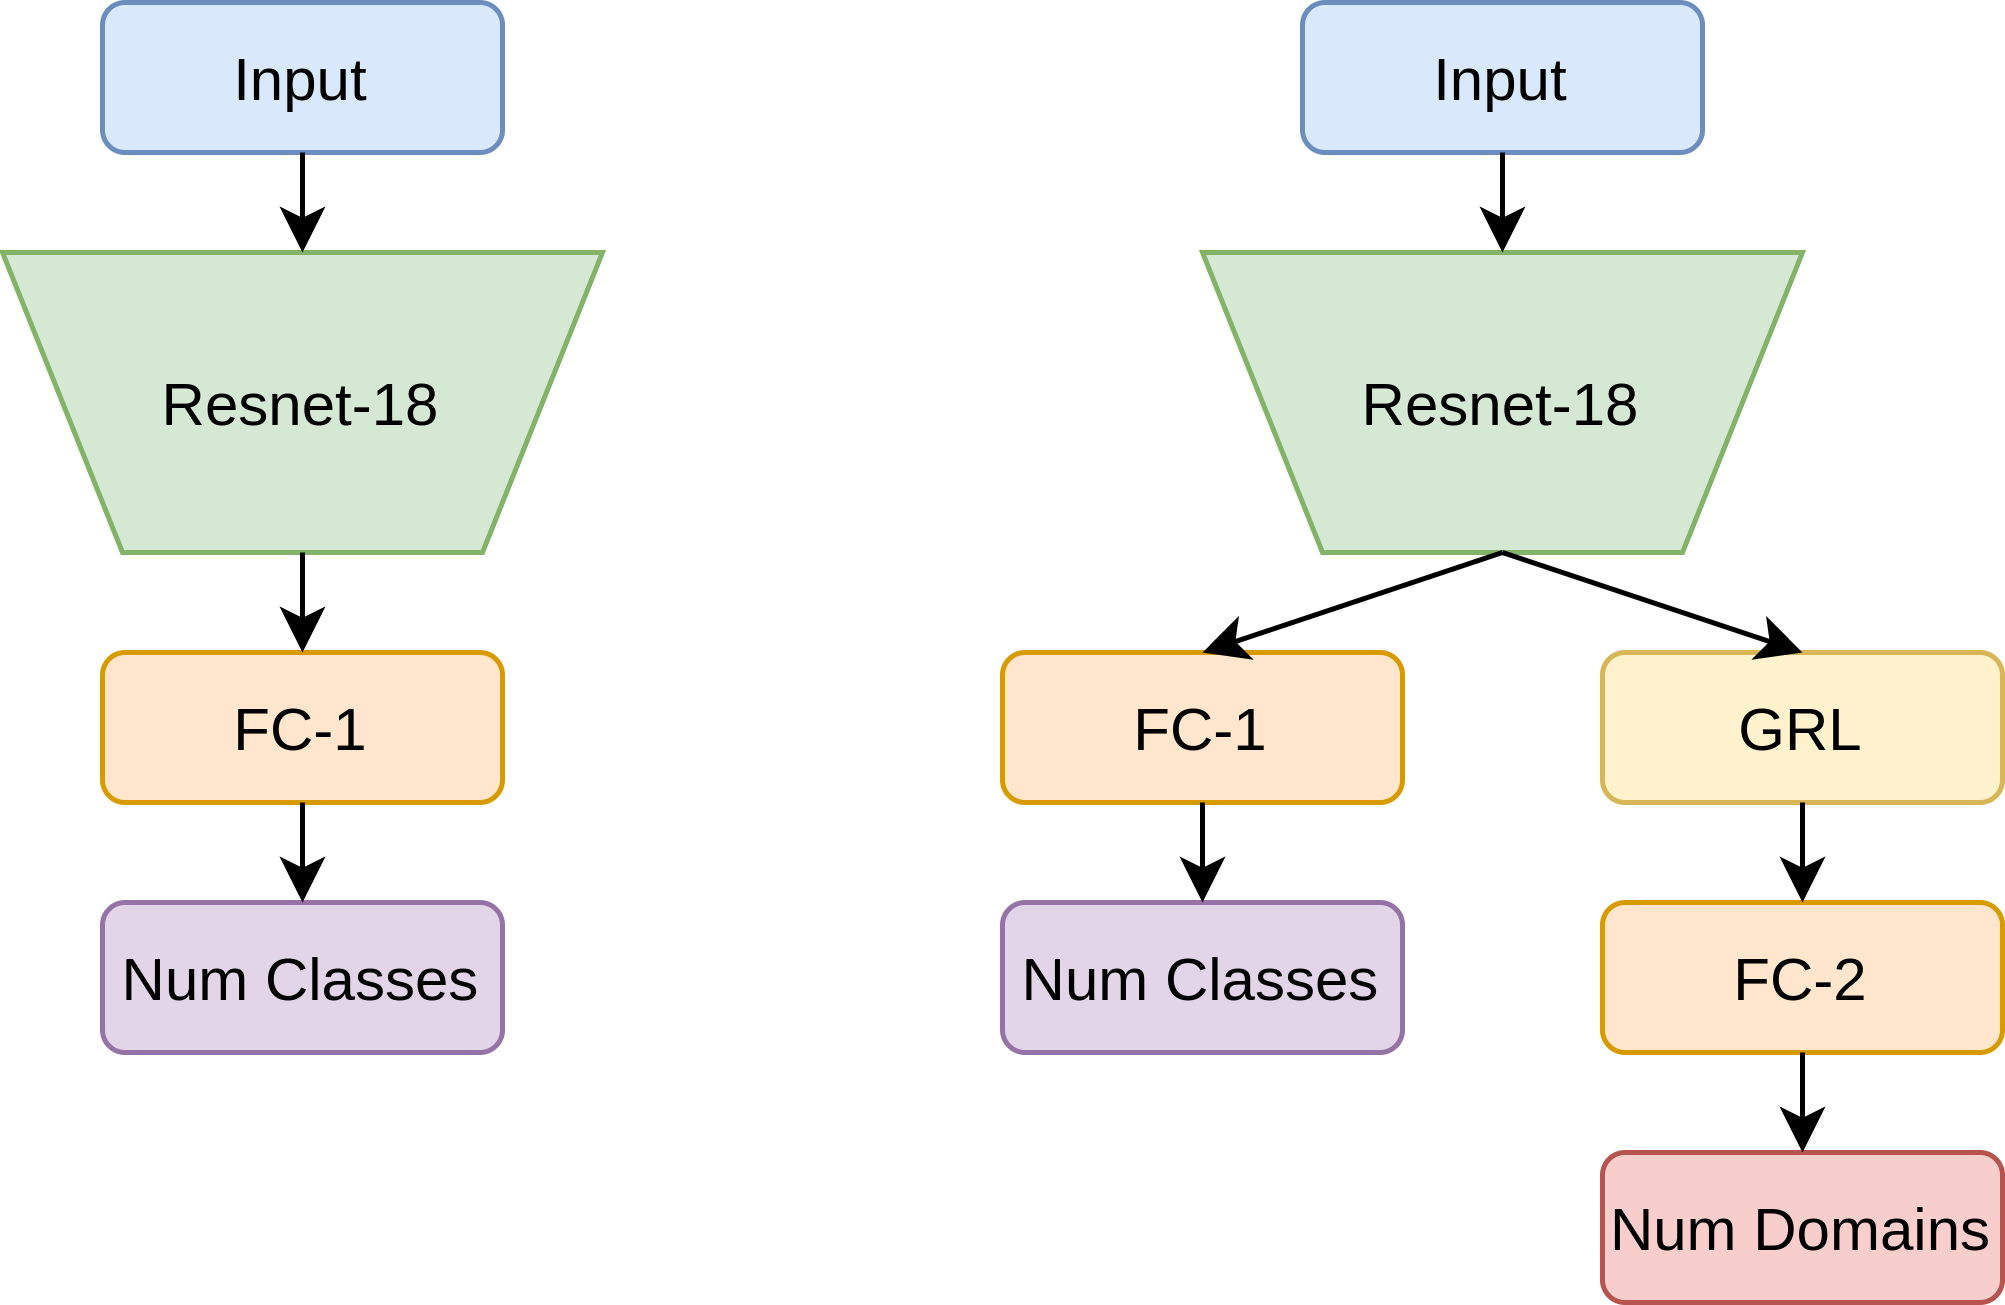
\includegraphics[width=\linewidth]{figures_supp/model.png} 
\caption{(Left) Supervised model architecture. (Right) Unsupervised model architecture.}
\label{model}
\end{figure}

\section{Experiment Embeddings}

We present the t-SNE embeddings for all our experiments in the section. 

%We find them inadequate at explaining the model behavior by themselves.

\begin{figure}[H]
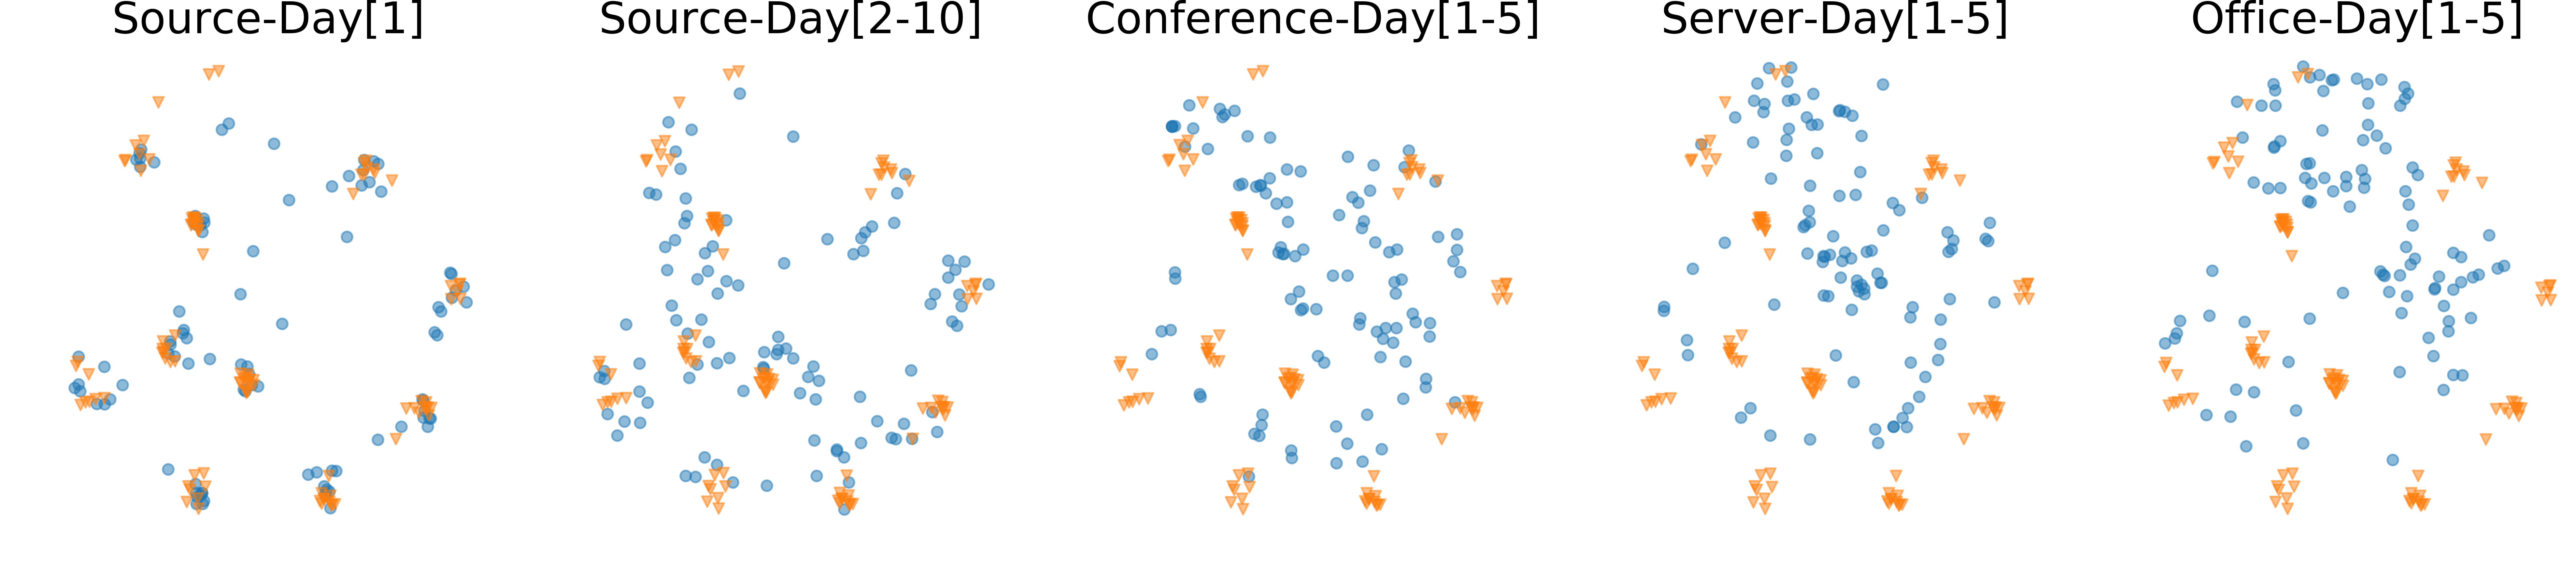
\includegraphics[width=\linewidth]{figures_supp/TargetLabelled100.png} 
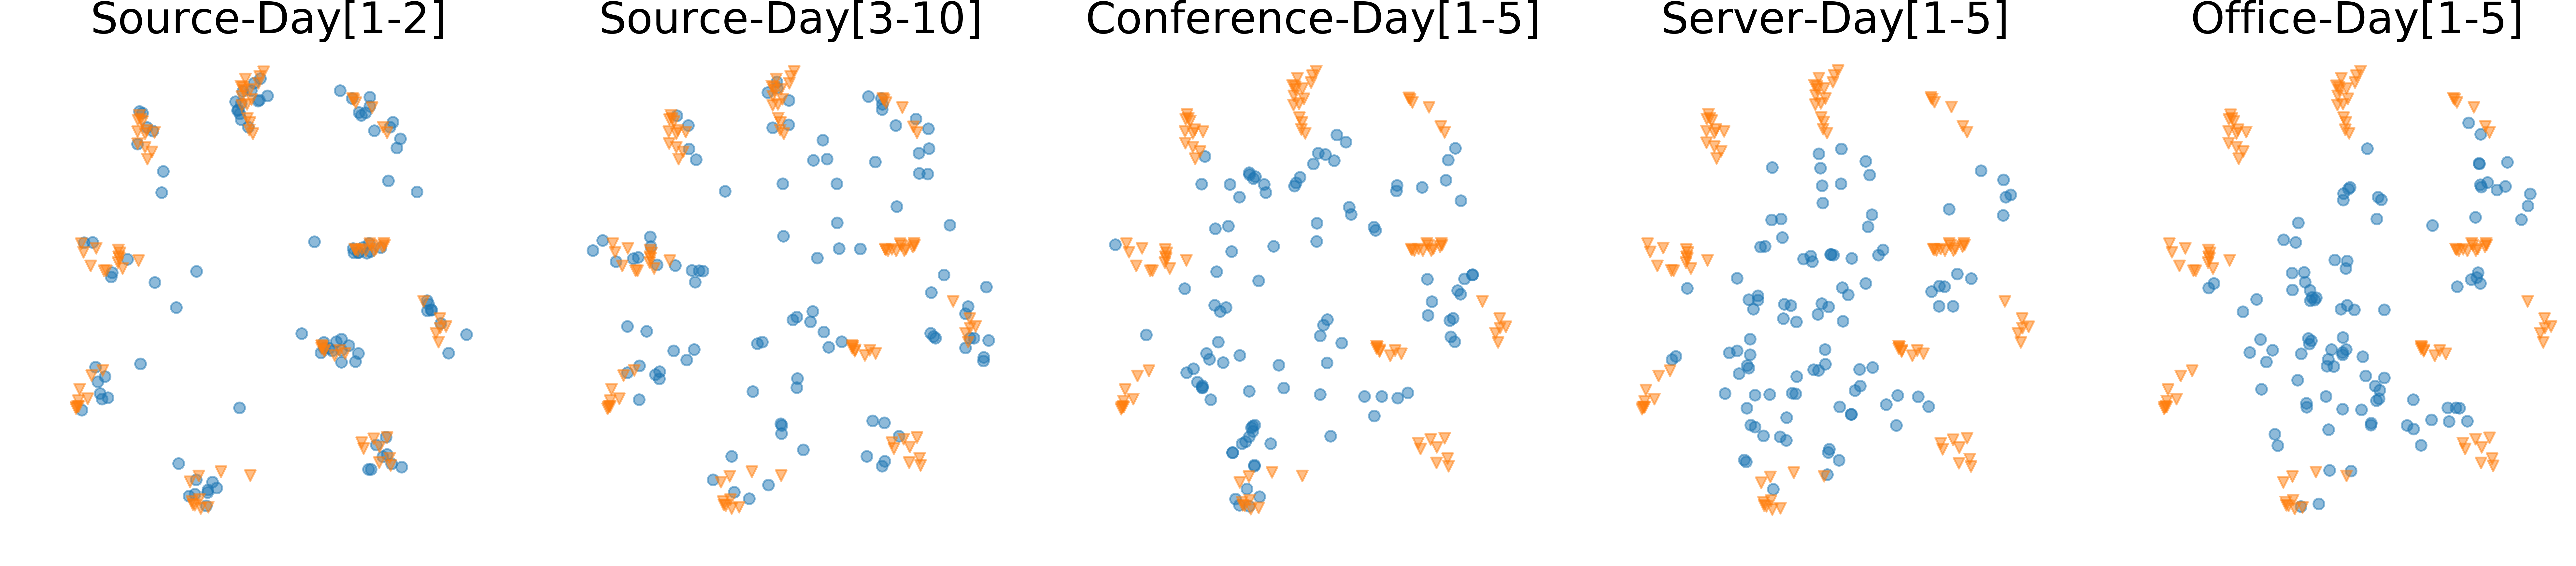
\includegraphics[width=\linewidth]{figures_supp/TargetLabelled200.png} 
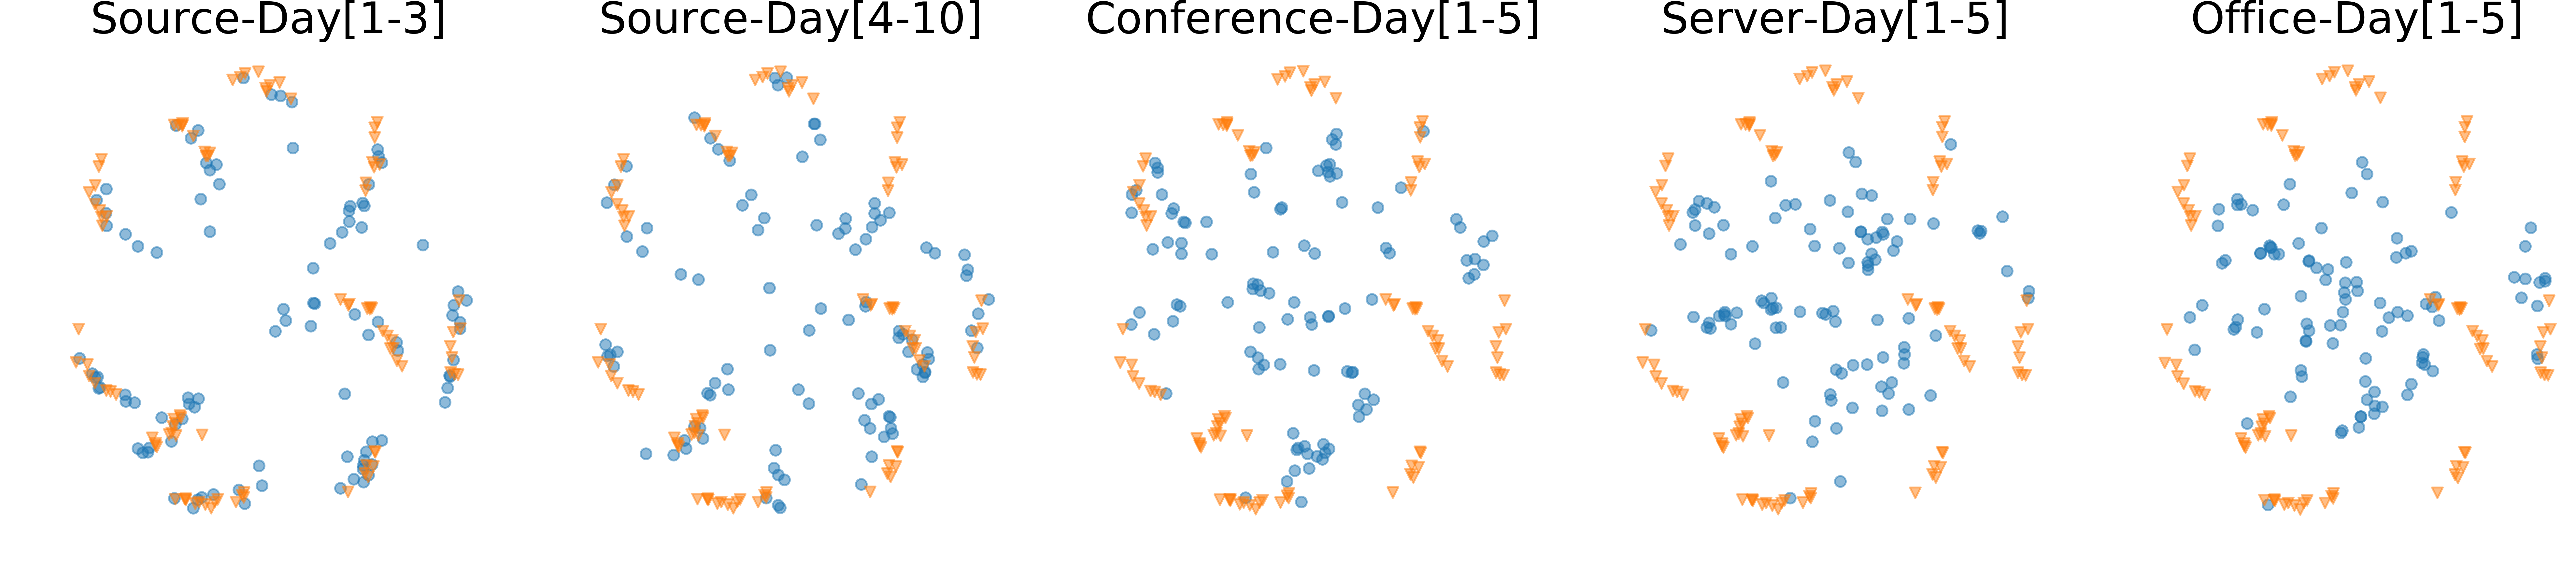
\includegraphics[width=\linewidth]{figures_supp/TargetLabelled300.png} 
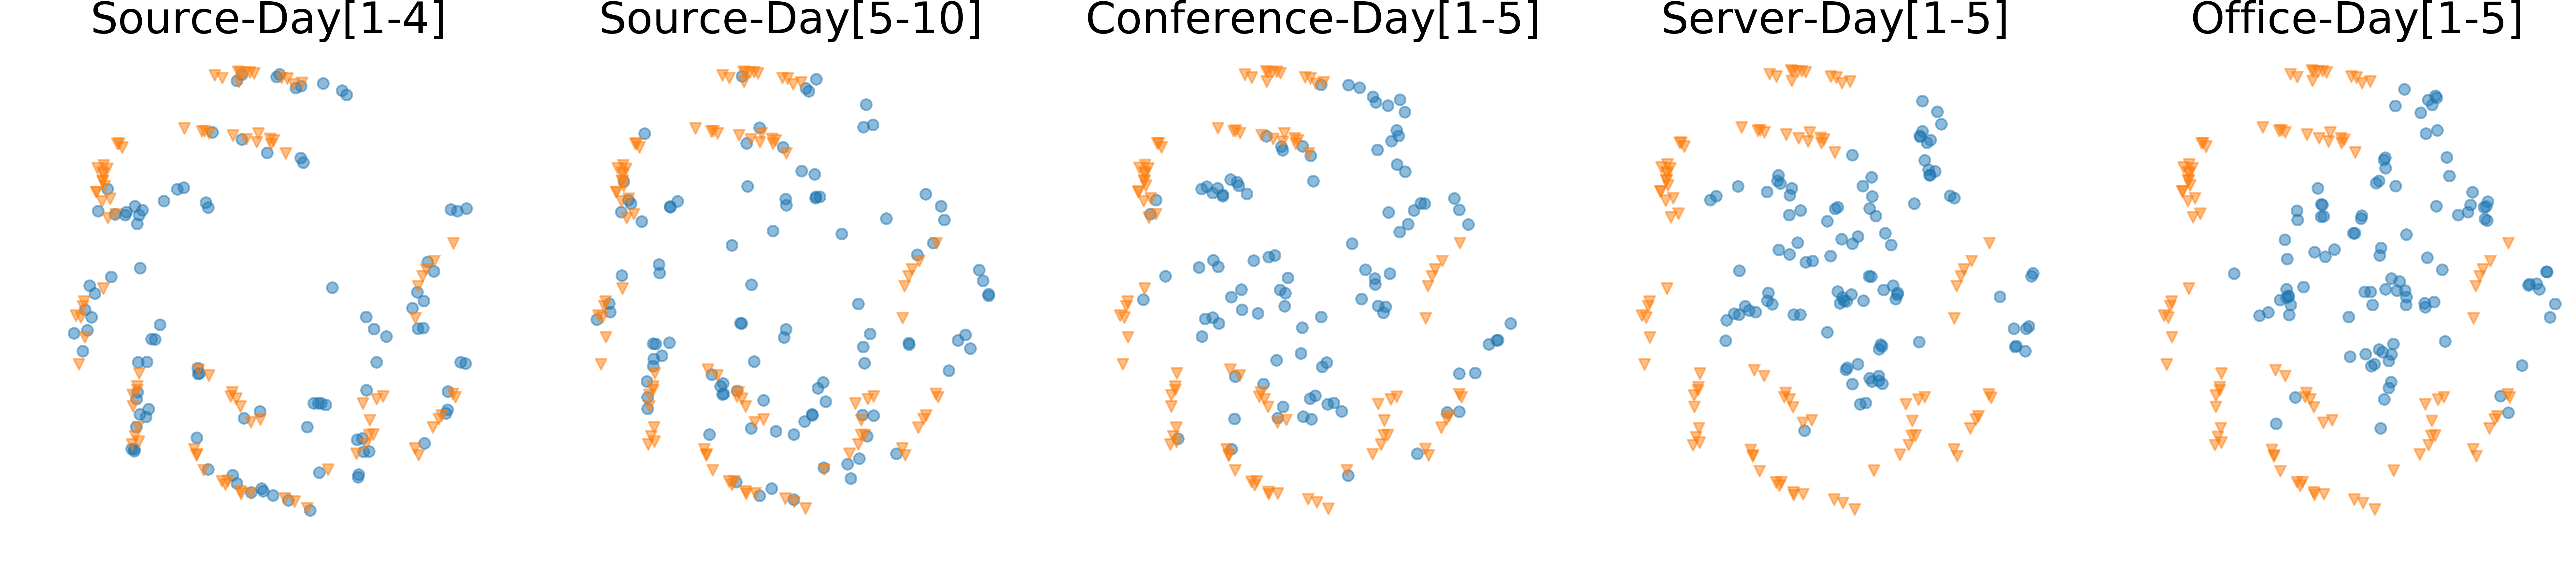
\includegraphics[width=\linewidth]{figures_supp/TargetLabelled400.png} 
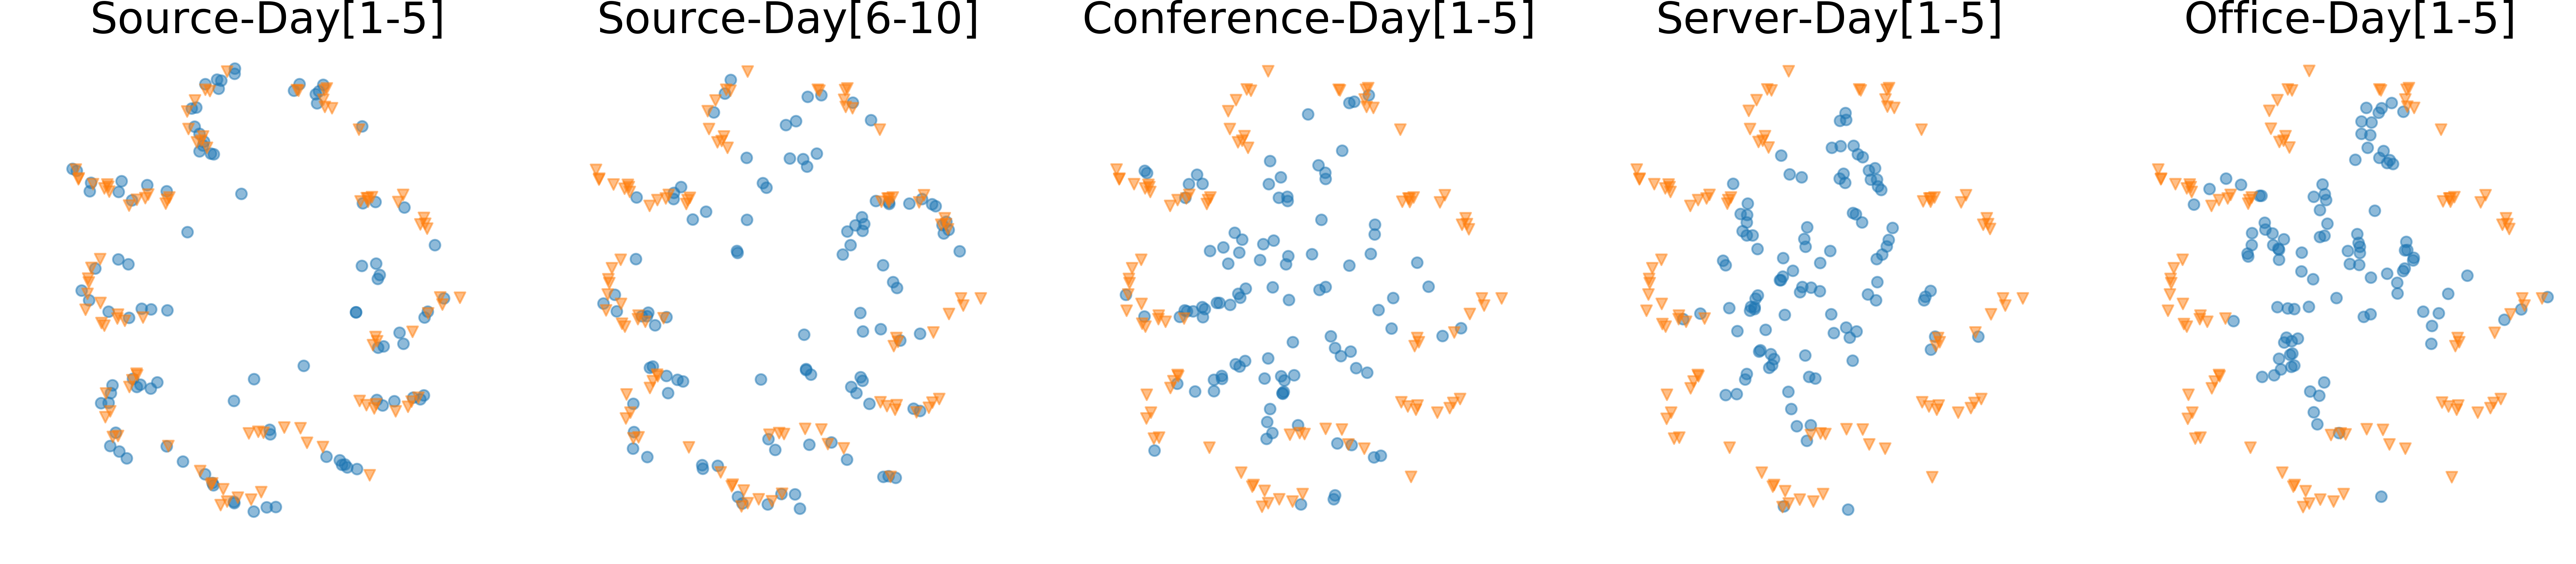
\includegraphics[width=\linewidth]{figures_supp/TargetLabelled500.png} 
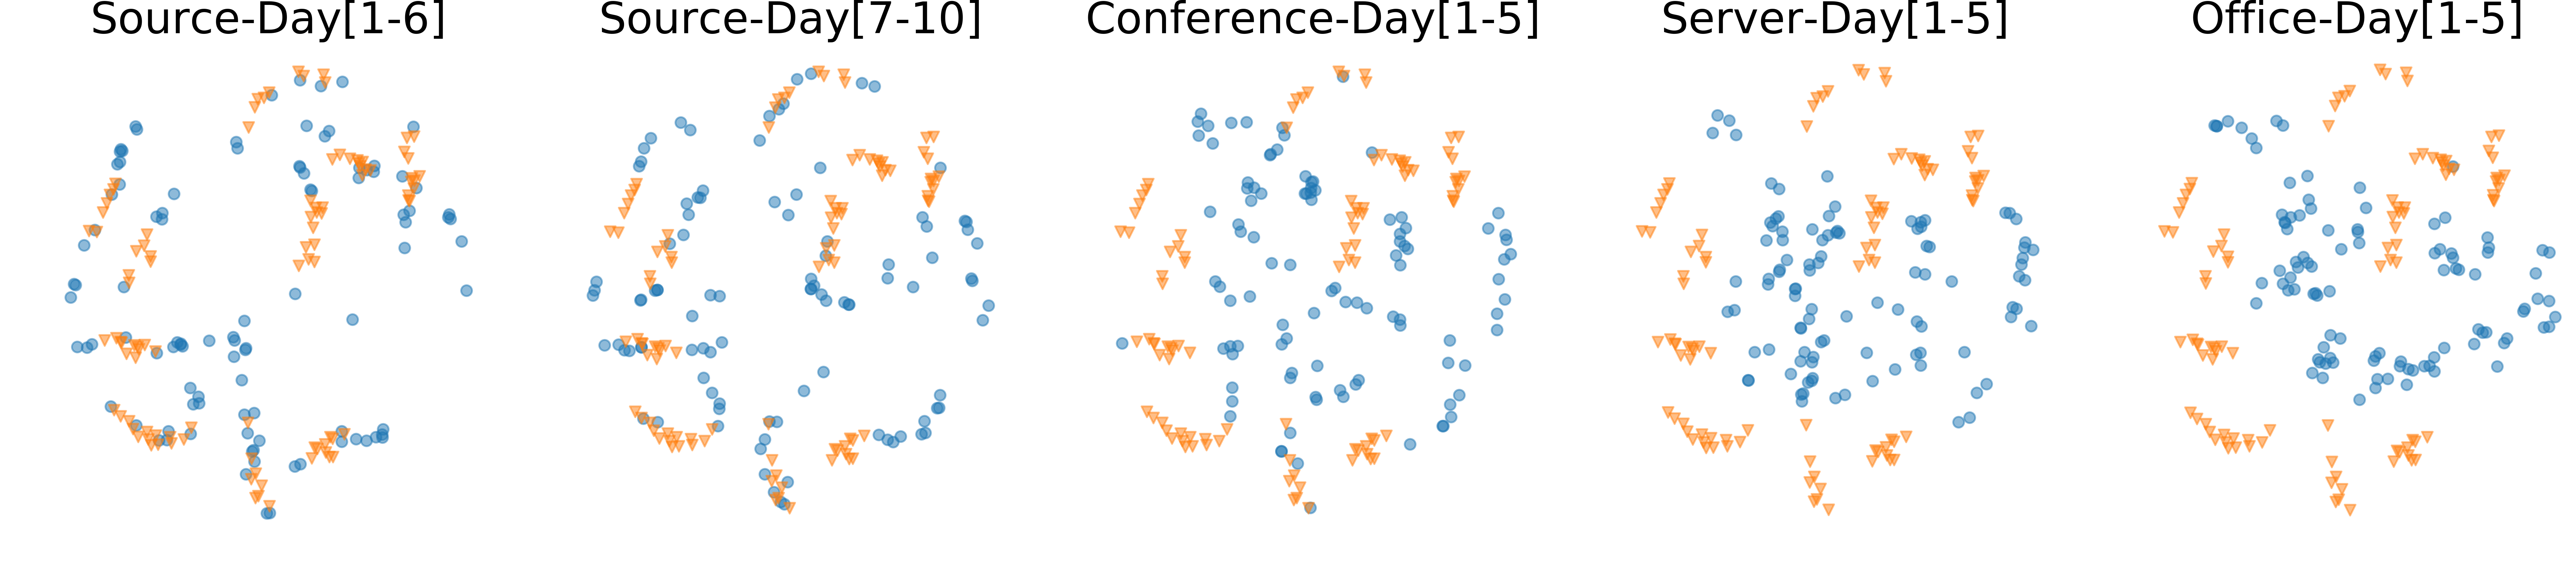
\includegraphics[width=\linewidth]{figures_supp/TargetLabelled600.png} 
\caption{Embeddings from the model trained using 1 to 6 days of source-only data. The number in brackets indicates the day indices. For example, [1 - 6] means the data from day 1 to day 6. Orange triangle clusters represent the training data (Source Location's Day 1), where each cluster represents a distinct human subject. Blue circles represent each domain’s testing data, where the data points were sampled from all the classes of a given domain. }
\label{scr1}
\end{figure}

\begin{figure}[H]
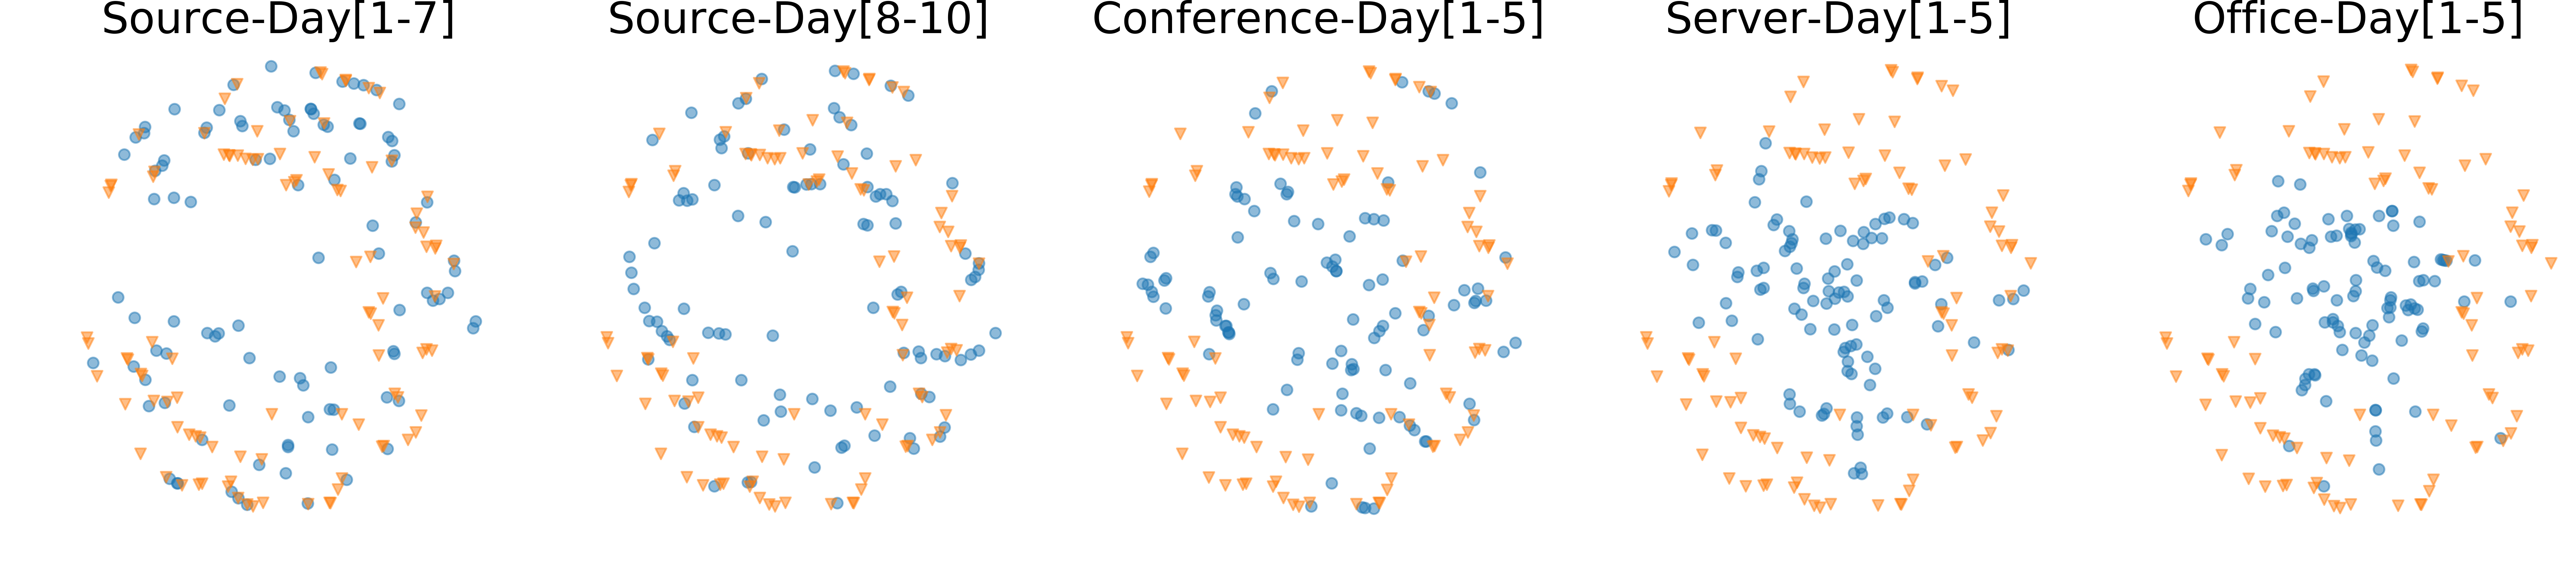
\includegraphics[width=\linewidth]{figures_supp/TargetLabelled700.png} 
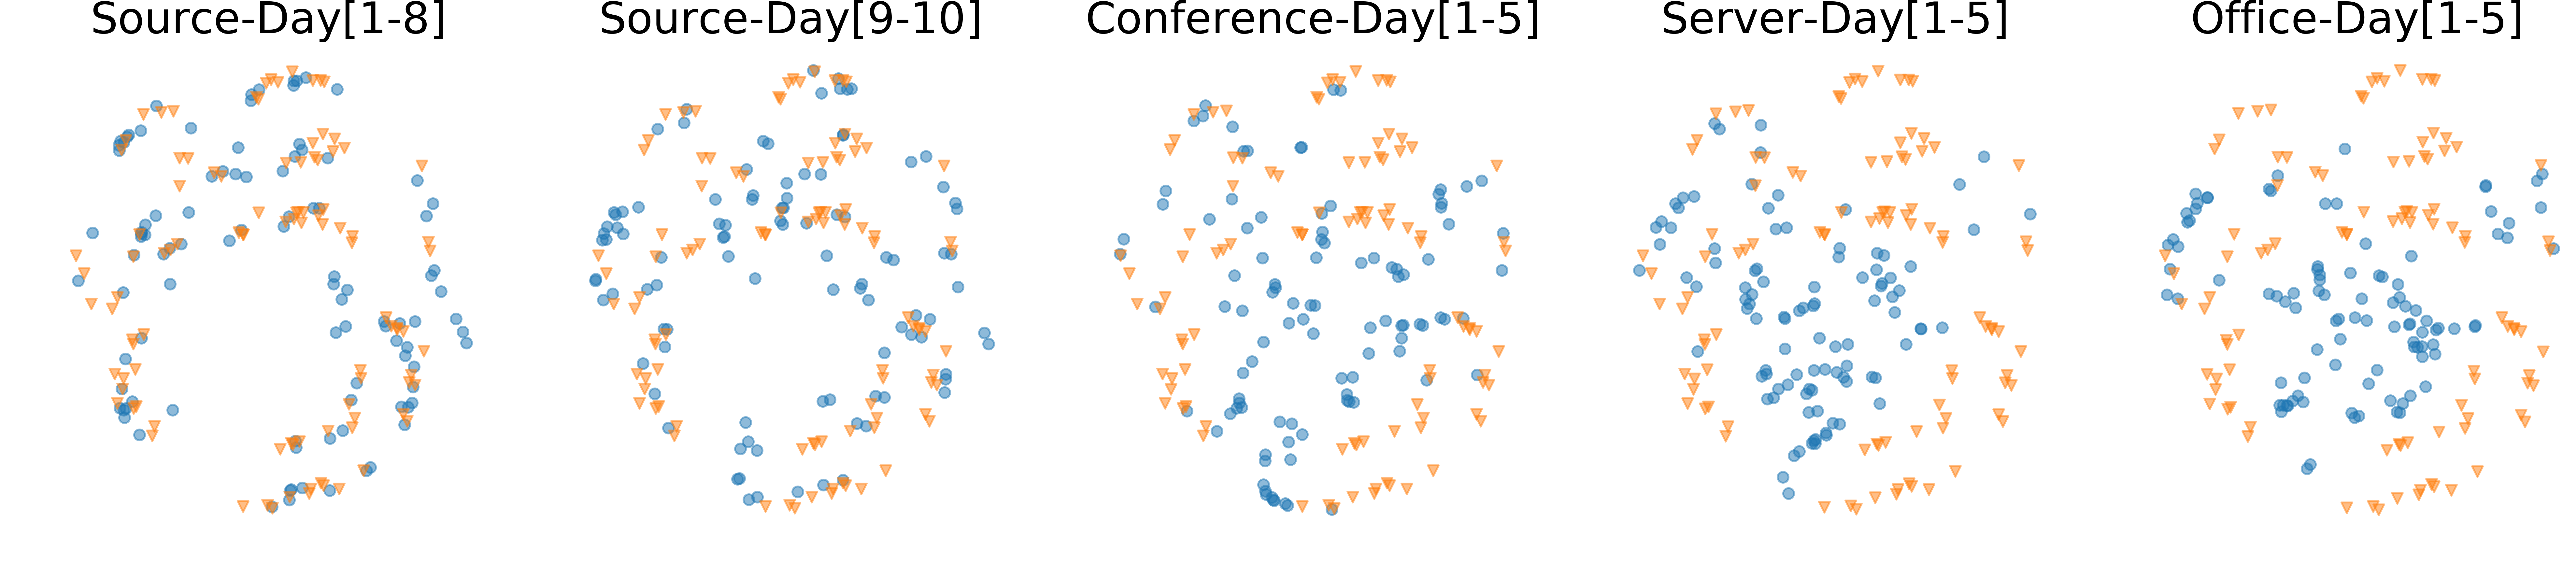
\includegraphics[width=\linewidth]{figures_supp/TargetLabelled800.png} 
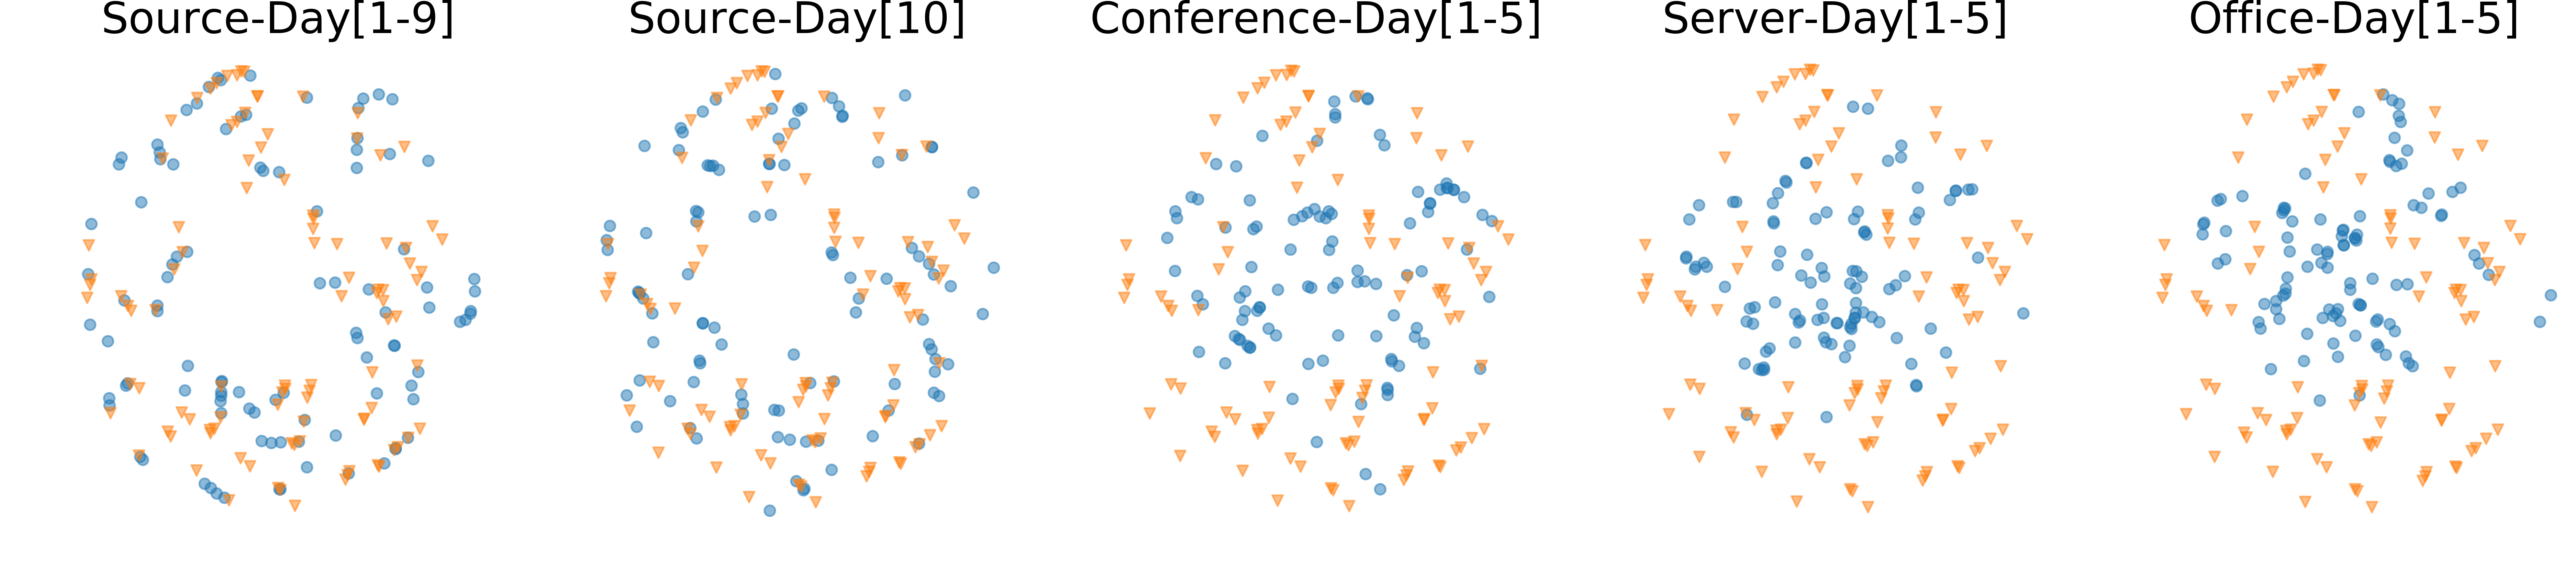
\includegraphics[width=\linewidth]{figures_supp/TargetLabelled900.png} 
\caption{Embeddings from the model trained using 7 to 9 days of source-only data}
\label{src2}
\end{figure}

\begin{figure}[H]
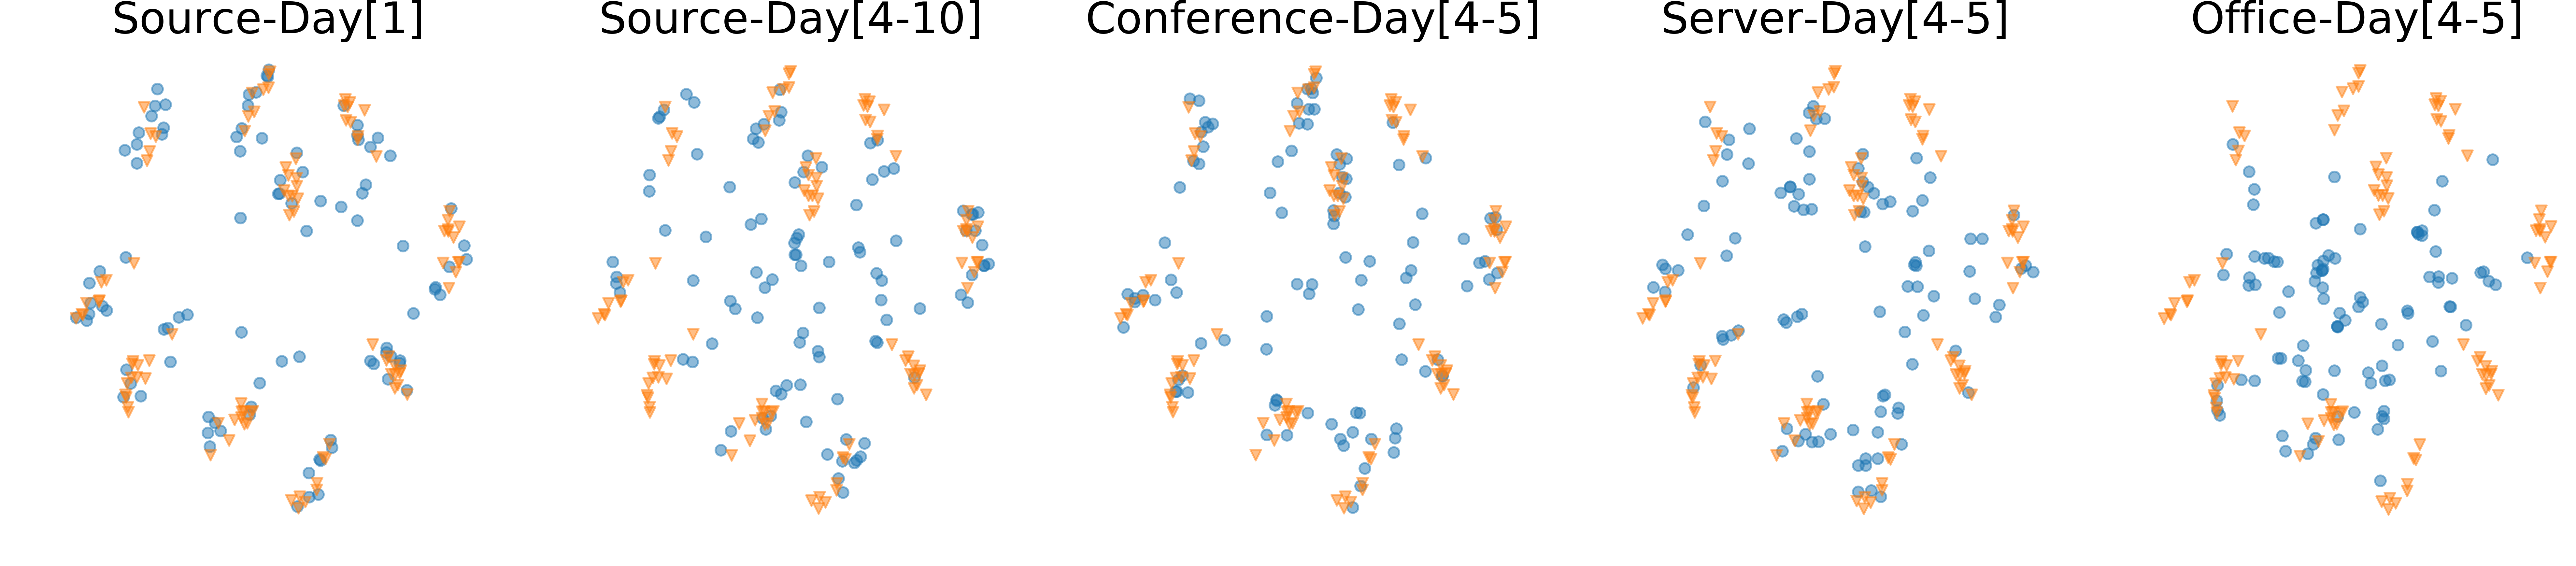
\includegraphics[width=\linewidth]{figures_supp/TargetLabelled111.png} 
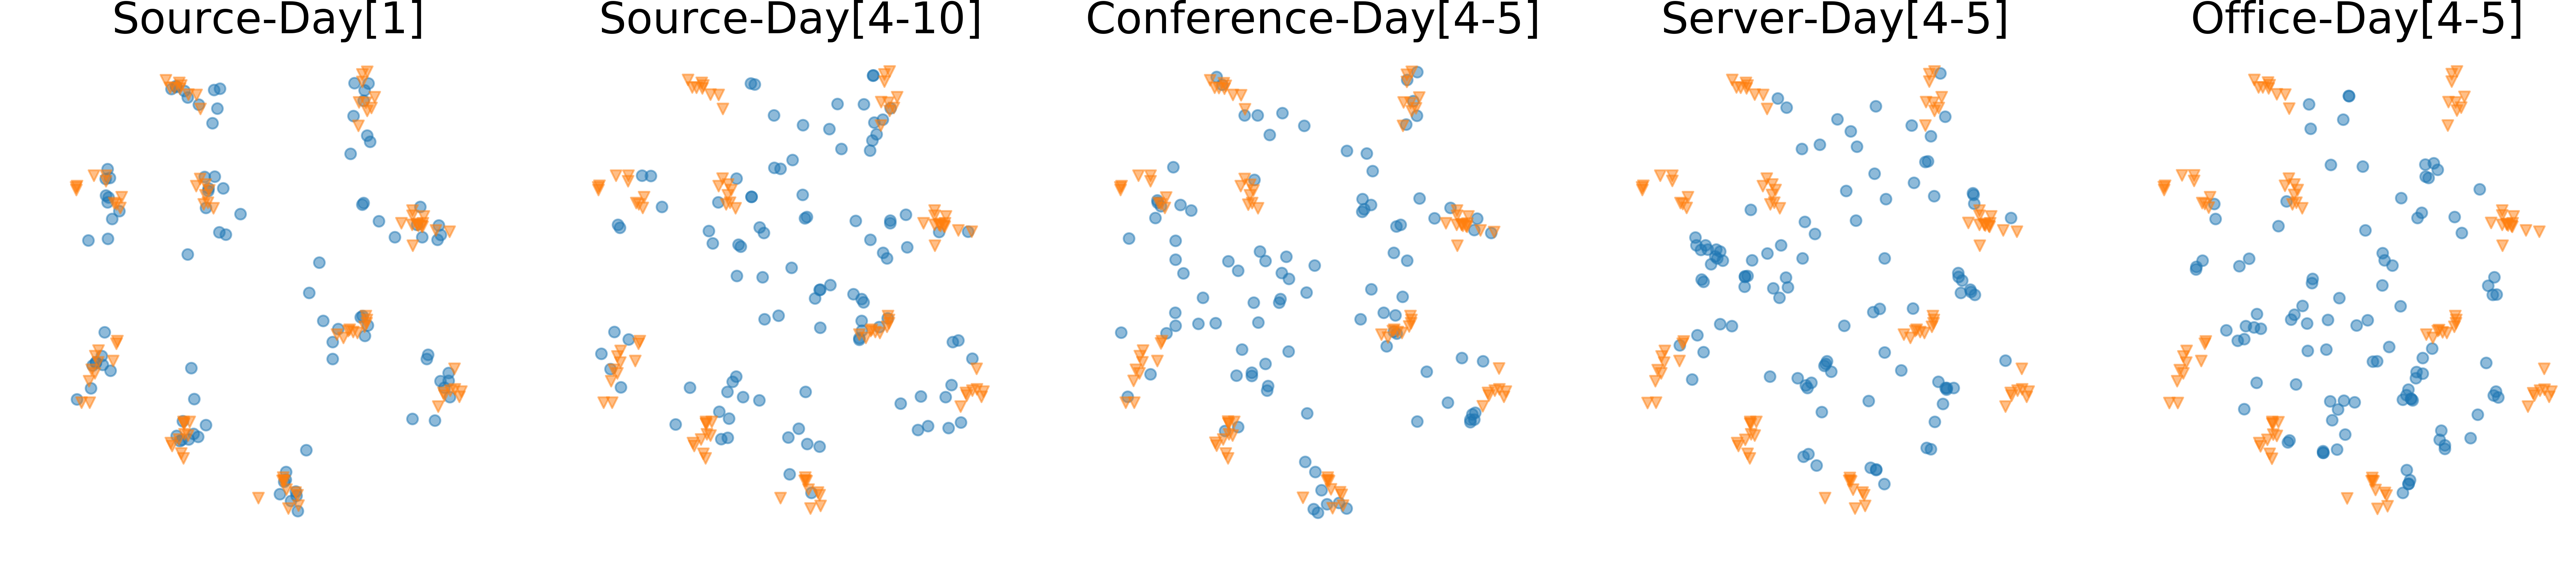
\includegraphics[width=\linewidth]{figures_supp/TargetLabelled101.png} 
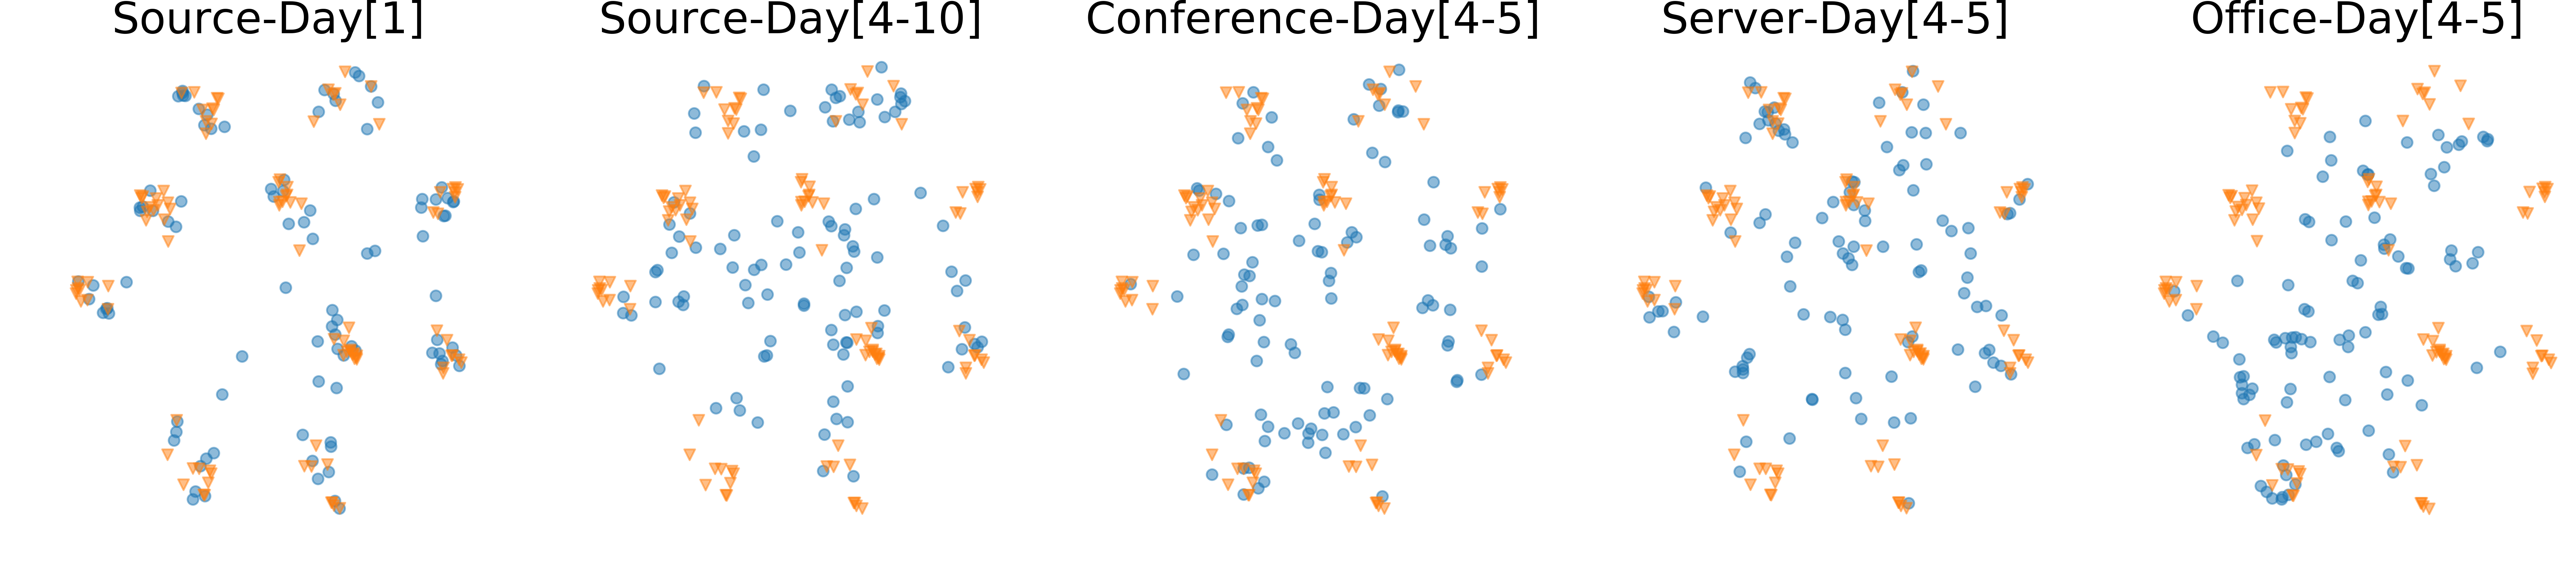
\includegraphics[width=\linewidth]{figures_supp/TargetLabelled110.png} 
\caption{Embeddings from model trained on source and target domain data. (Top) model trained one day of source, server and conference data, (Middle) model trained via one day of source and conference data, (Bottom) model trained via one day of source and server data}
\label{trg1}
\end{figure}

\begin{figure}[H]
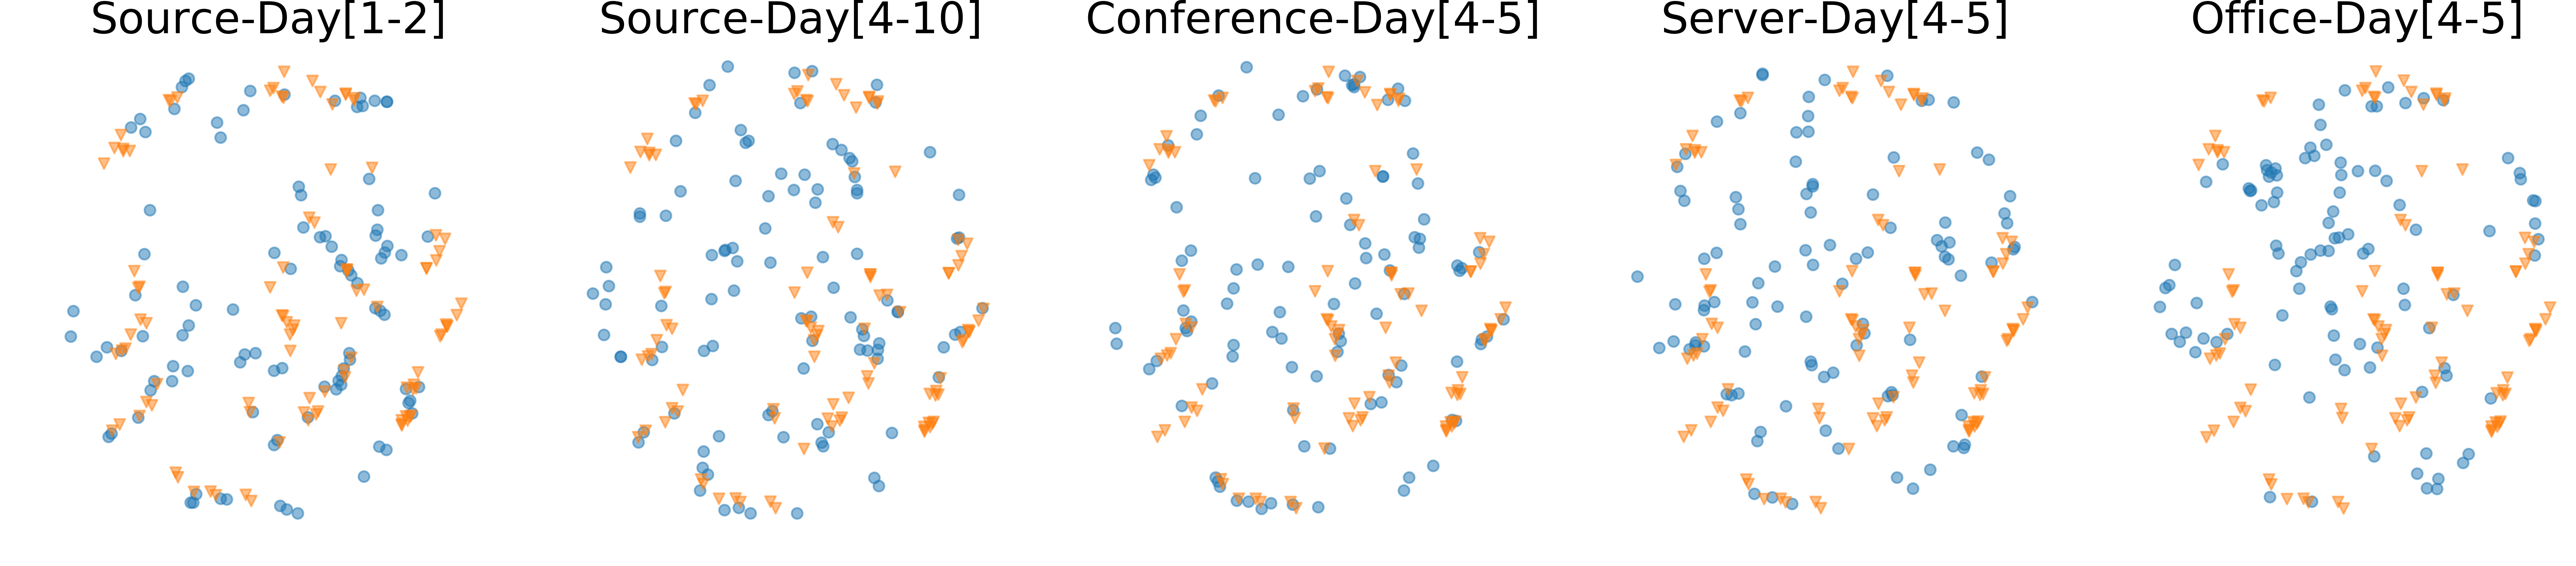
\includegraphics[width=\linewidth]{figures_supp/TargetLabelled222.png} 
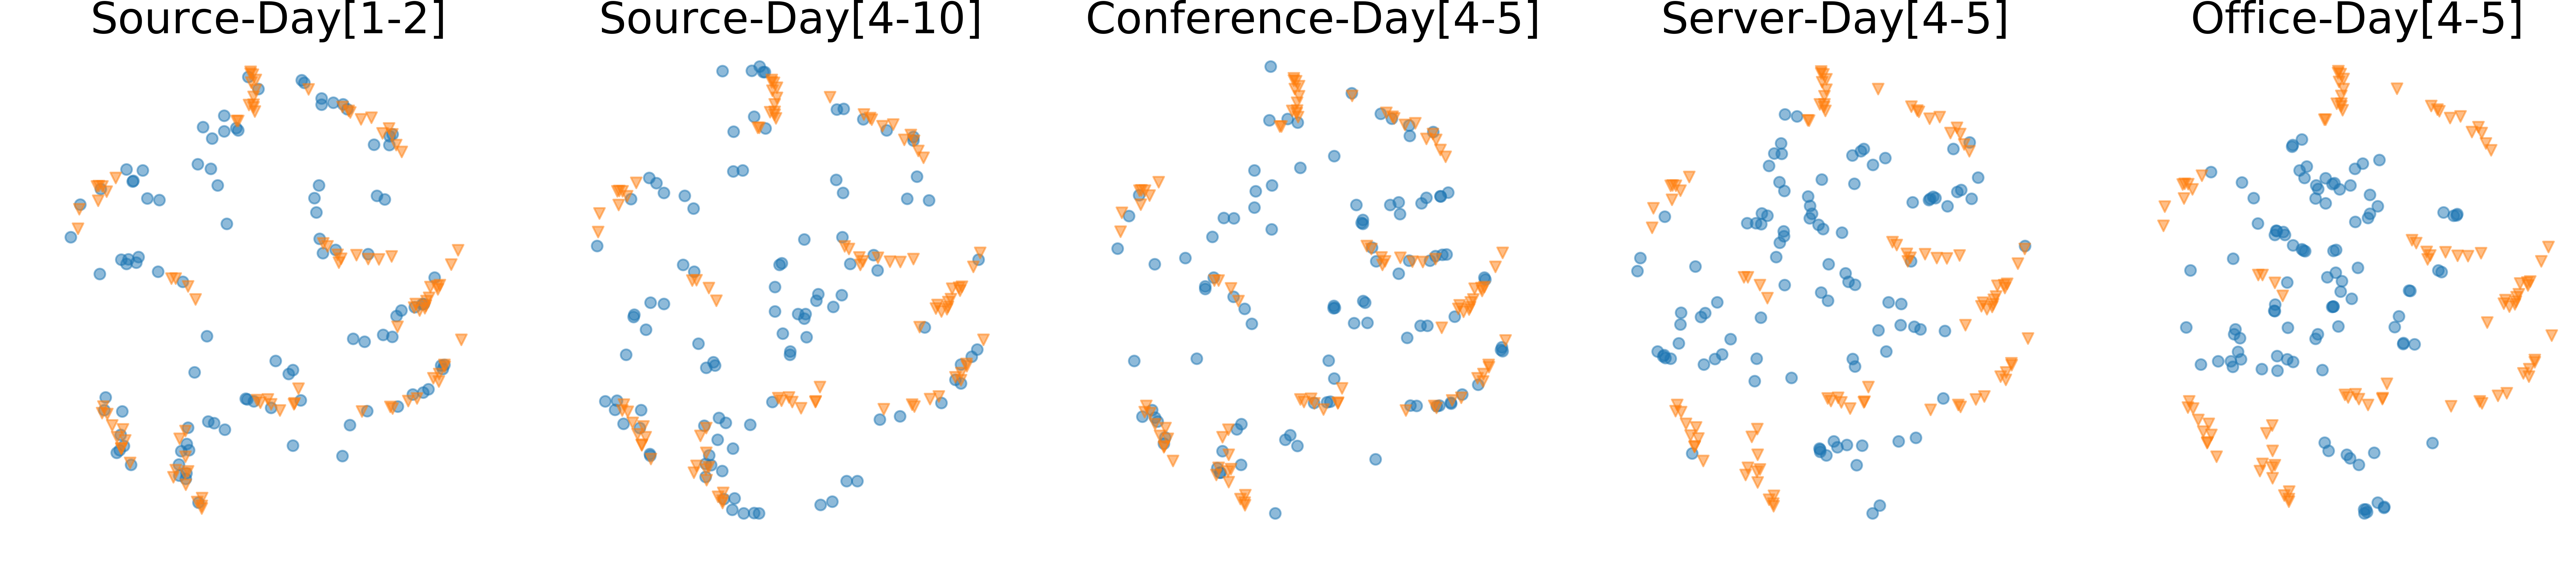
\includegraphics[width=\linewidth]{figures_supp/TargetLabelled202.png} 
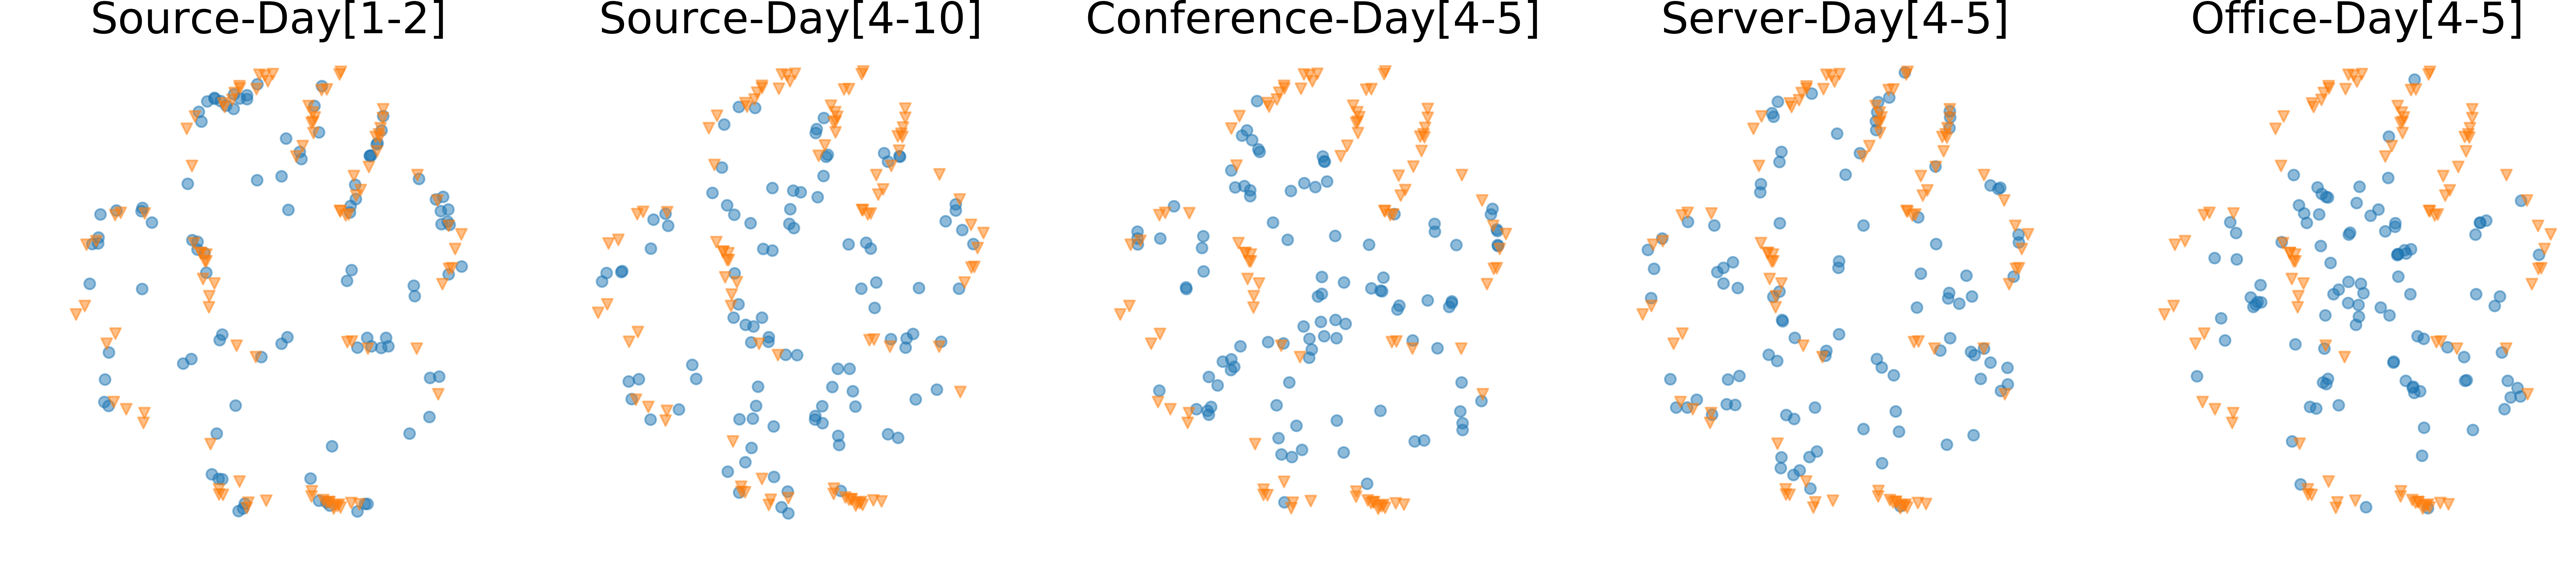
\includegraphics[width=\linewidth]{figures_supp/TargetLabelled220.png} 
\caption{Embeddings from model trained on source and target domain data. (Top) model trained via two days of source, server and conference data, (Middle) model trained via two days of source and conference data, (Bottom) model trained via two days of source and server data}
\label{trg2}
\end{figure}

\begin{figure}[H]
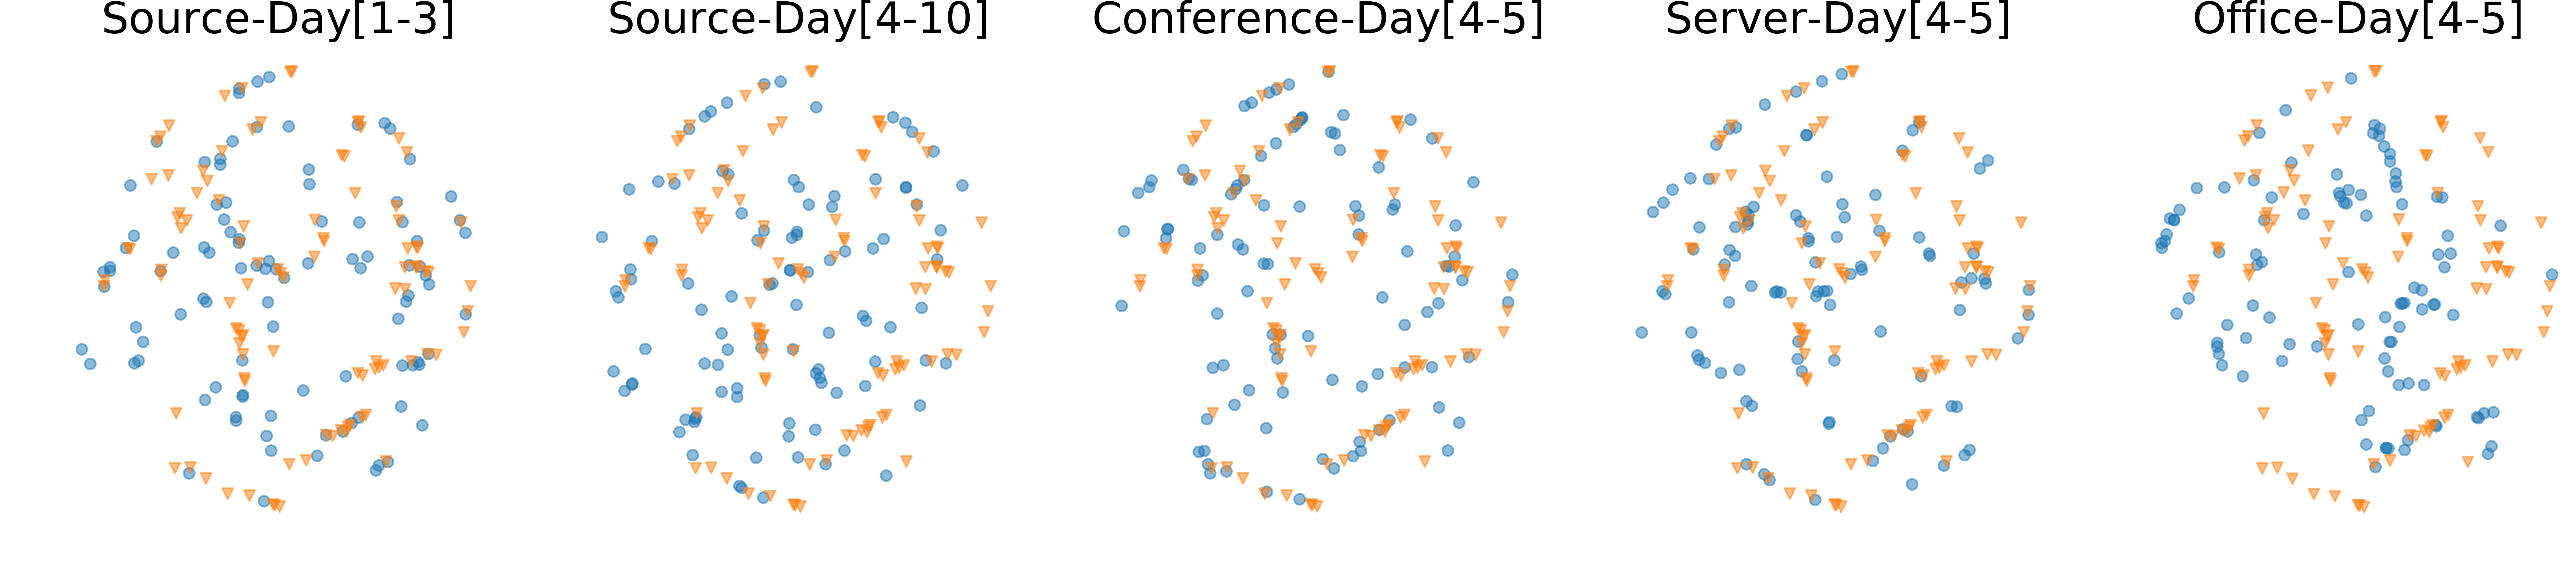
\includegraphics[width=\linewidth]{figures_supp/TargetLabelled333.png} 
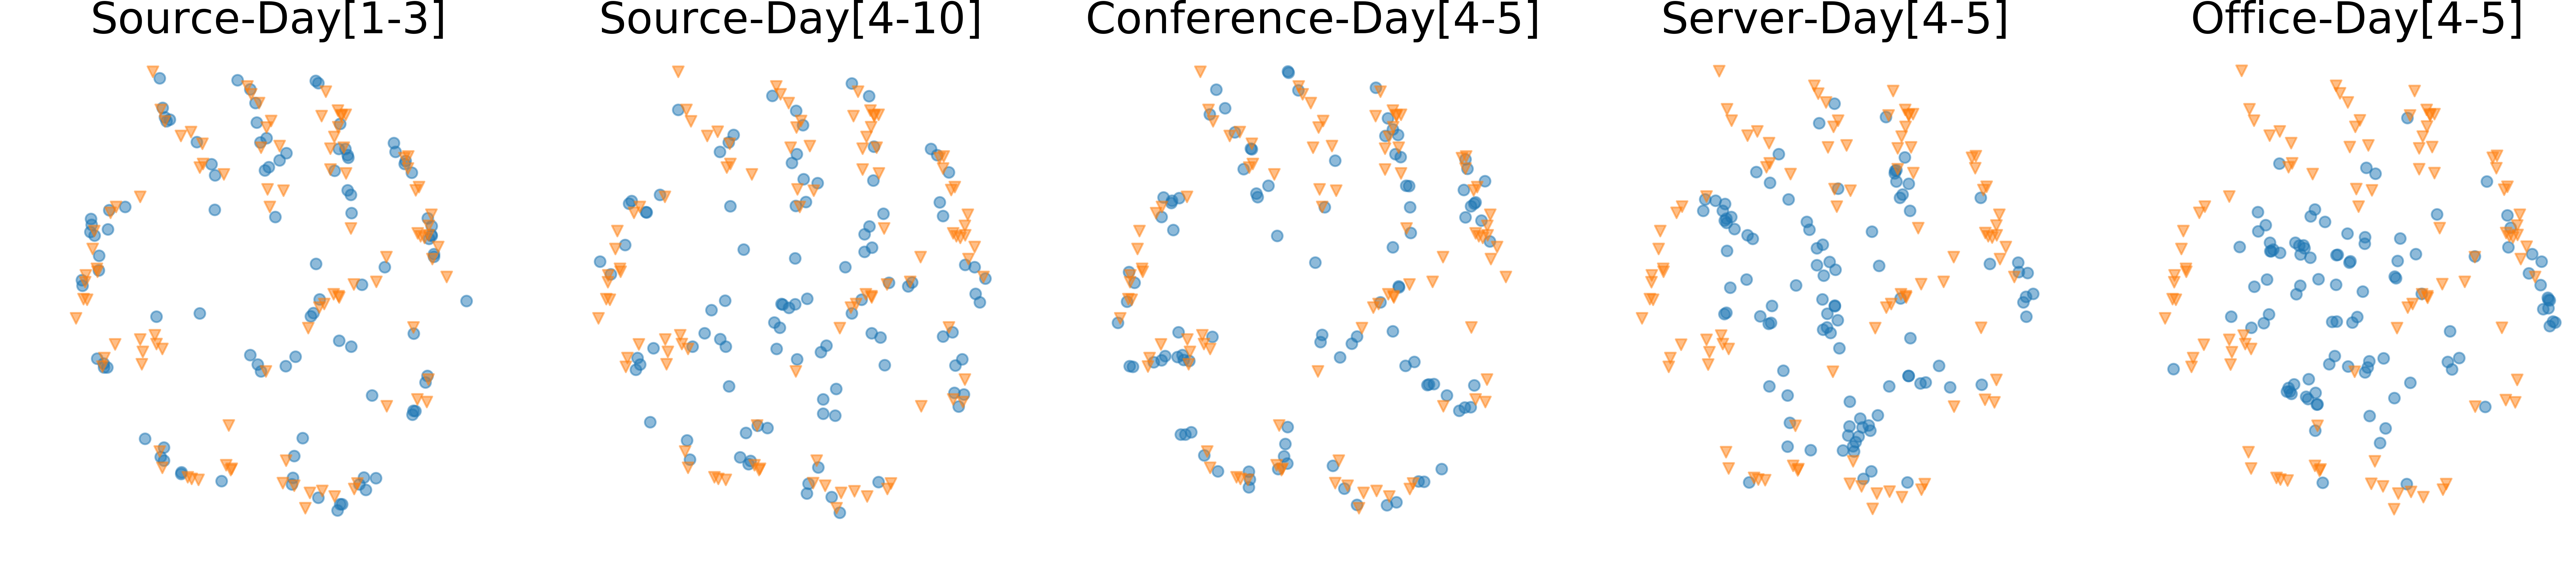
\includegraphics[width=\linewidth]{figures_supp/TargetLabelled303.png} 
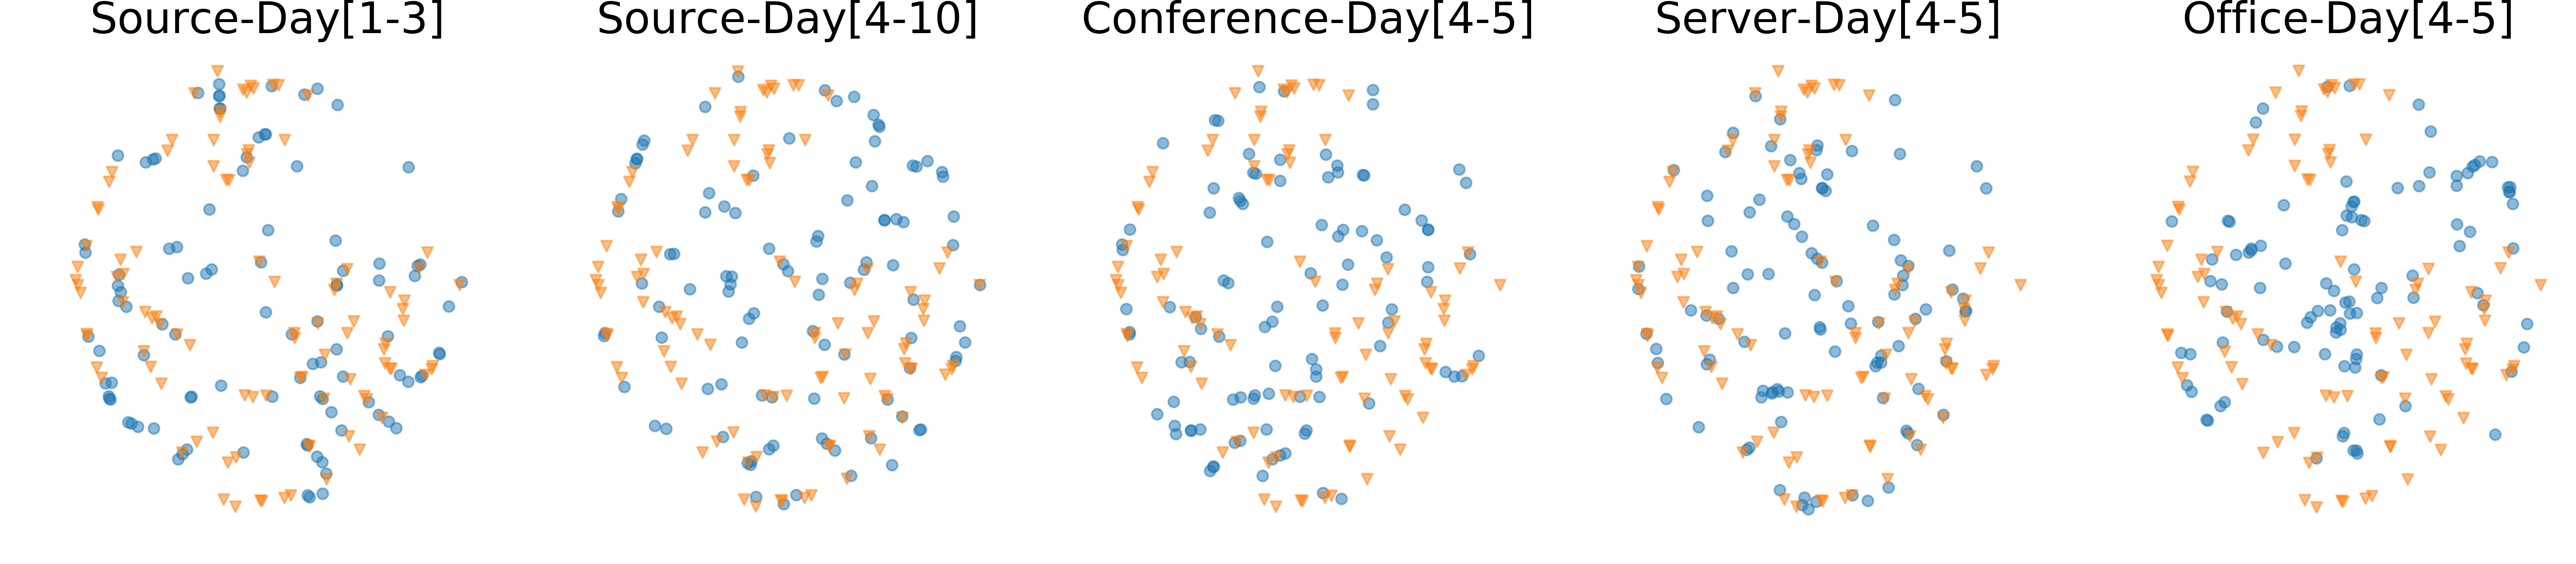
\includegraphics[width=\linewidth]{figures_supp/TargetLabelled330.png} 
\caption{Embeddings from model trained on source and target domain data. (Top) model trained via three days of source, server and conference data, (Middle) model trained via three days of source and conference data, (Bottom) model trained via three days of source and server data}
\label{trg3}
\end{figure}

\begin{figure}[H]
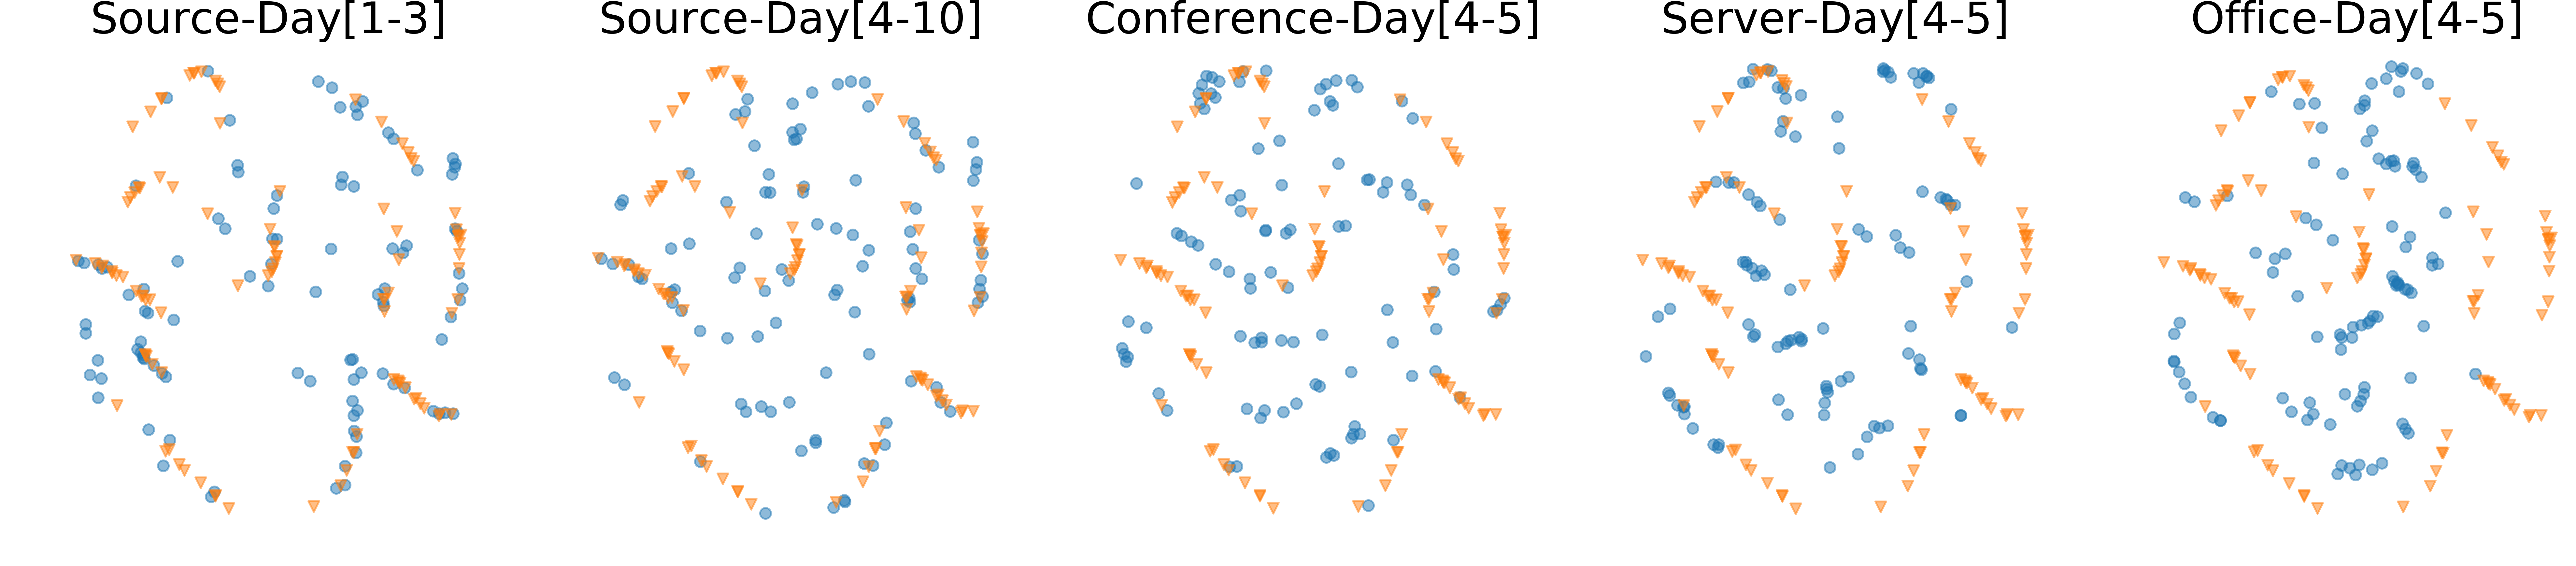
\includegraphics[width=\linewidth]{figures_supp/TargetUnLabelled330.png} 
\caption{Embeddings from model trained on three days of labeled source and three days of unlabeled server domain data. The unsupervised data was trained using a GAN based approach.}
\label{uda}
\end{figure}

\section{Experiment Shift Metrics}

Here we present the accuracies obtained from all our experiments alongside the corresponding metric learning based distance metrics. We find that not only does the distance metrics agree with the accuracy based findings, it also makes it more evident. Indeed we see an apparent temporal degradation in Fig.~\ref{srconly} in the source domain. Moreover, introducing more training data from the source domain alleviates the SDS to a certain extent, but it also biases the model more towards the source domain in some cases.

\begin{figure}[H]
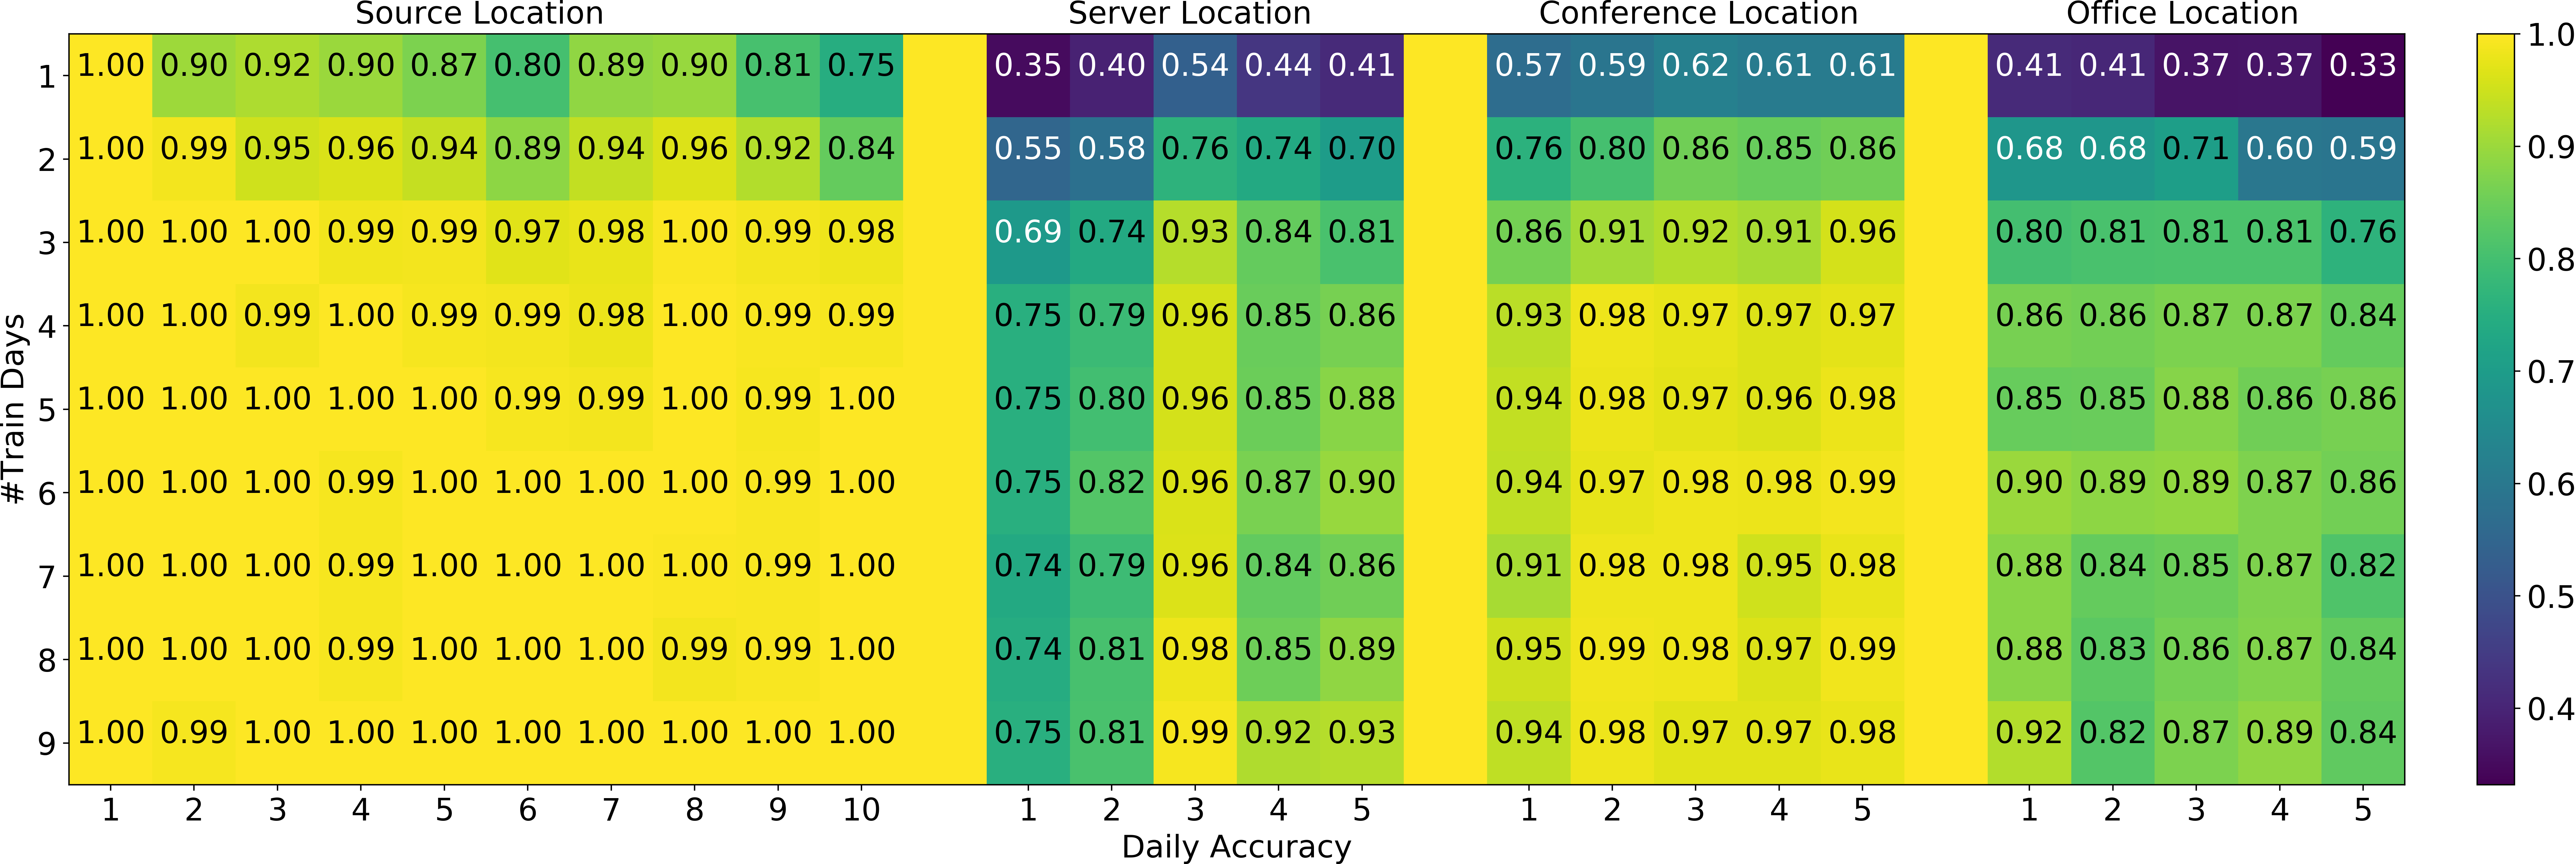
\includegraphics[width=\linewidth]{figures_supp/Exp1.png} 
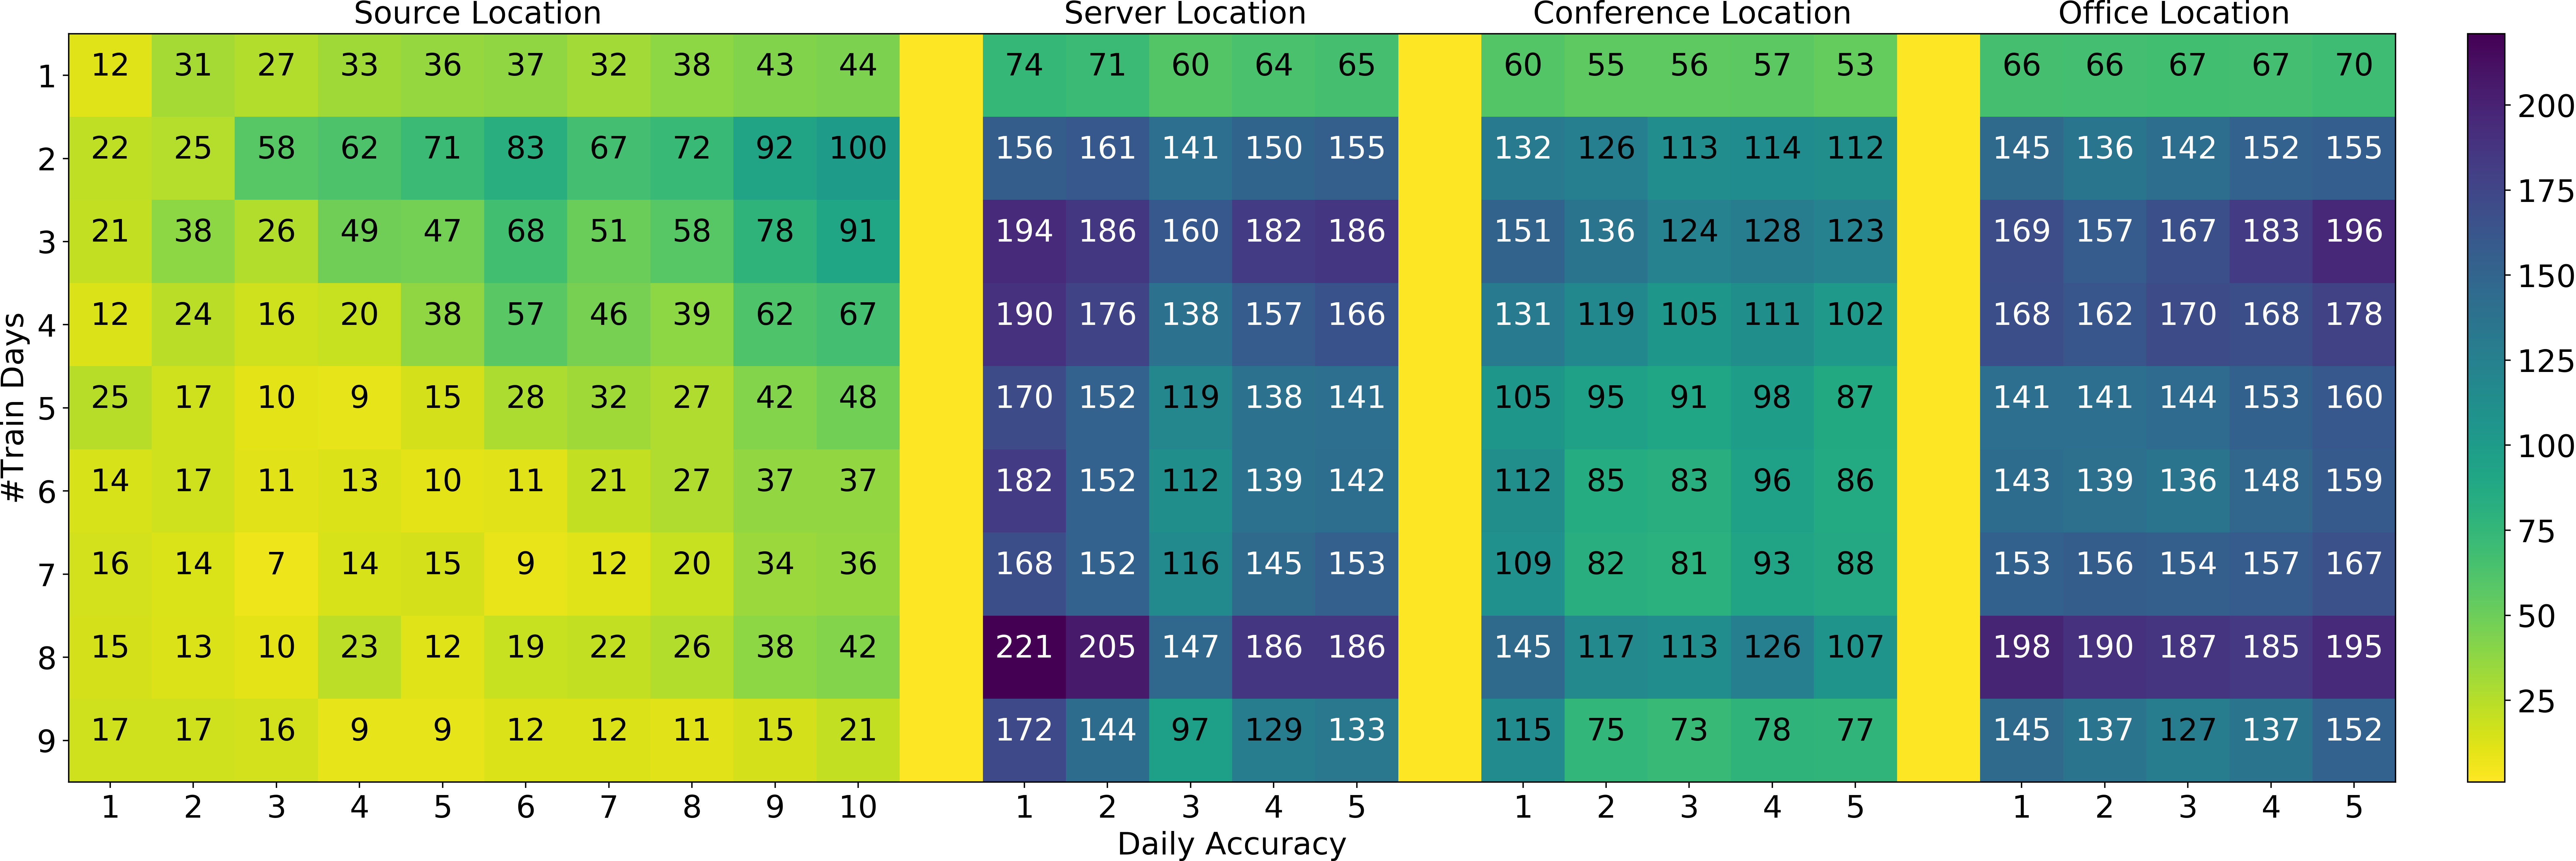
\includegraphics[width=\linewidth]{figures_supp/Exp1-metric.png} 
\caption{Results obtained from training only on source location data for varying number of days.}
\label{srconly}
\end{figure}

\begin{figure}[H]
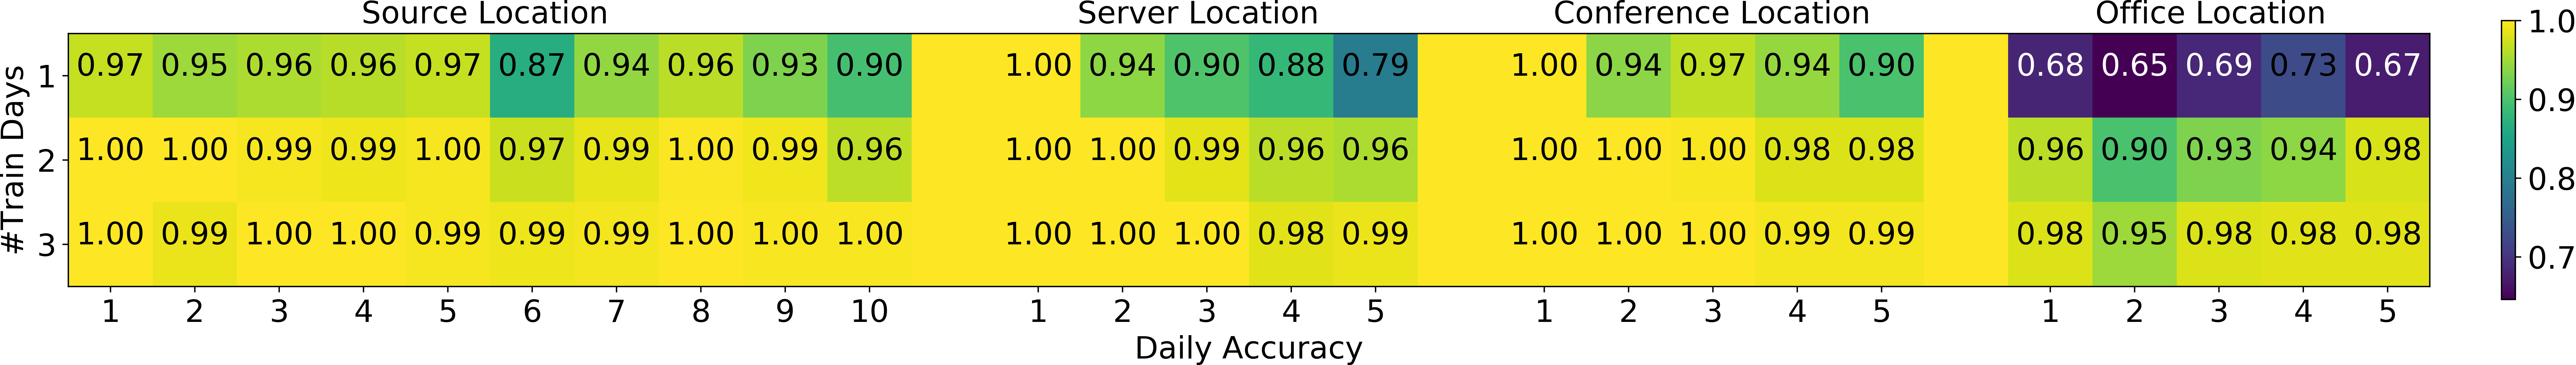
\includegraphics[width=\linewidth]{figures_supp/Exp2.png} 
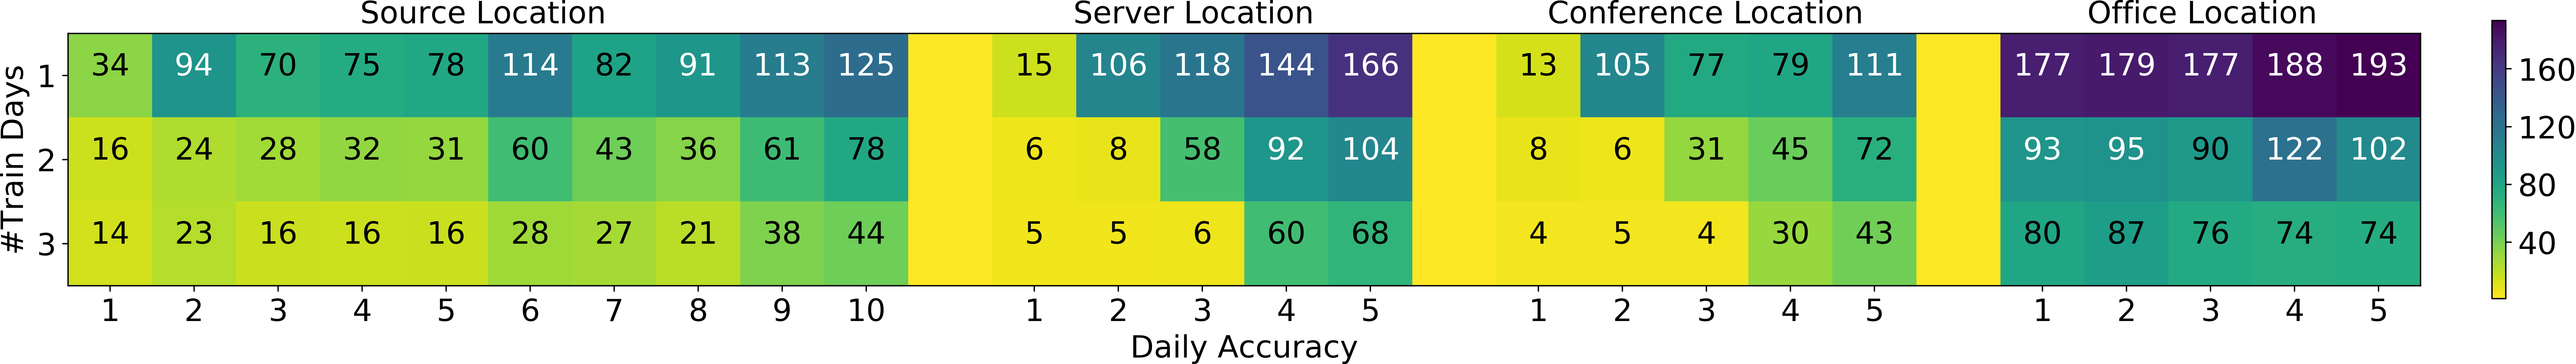
\includegraphics[width=\linewidth]{figures_supp/Exp4.png} 
\caption{Results obtained from training on source, server, and conference location data for varying number of days. The data from office location is not used for training and only for testing}
\label{srctrg}
\end{figure}

\begin{figure}[H]
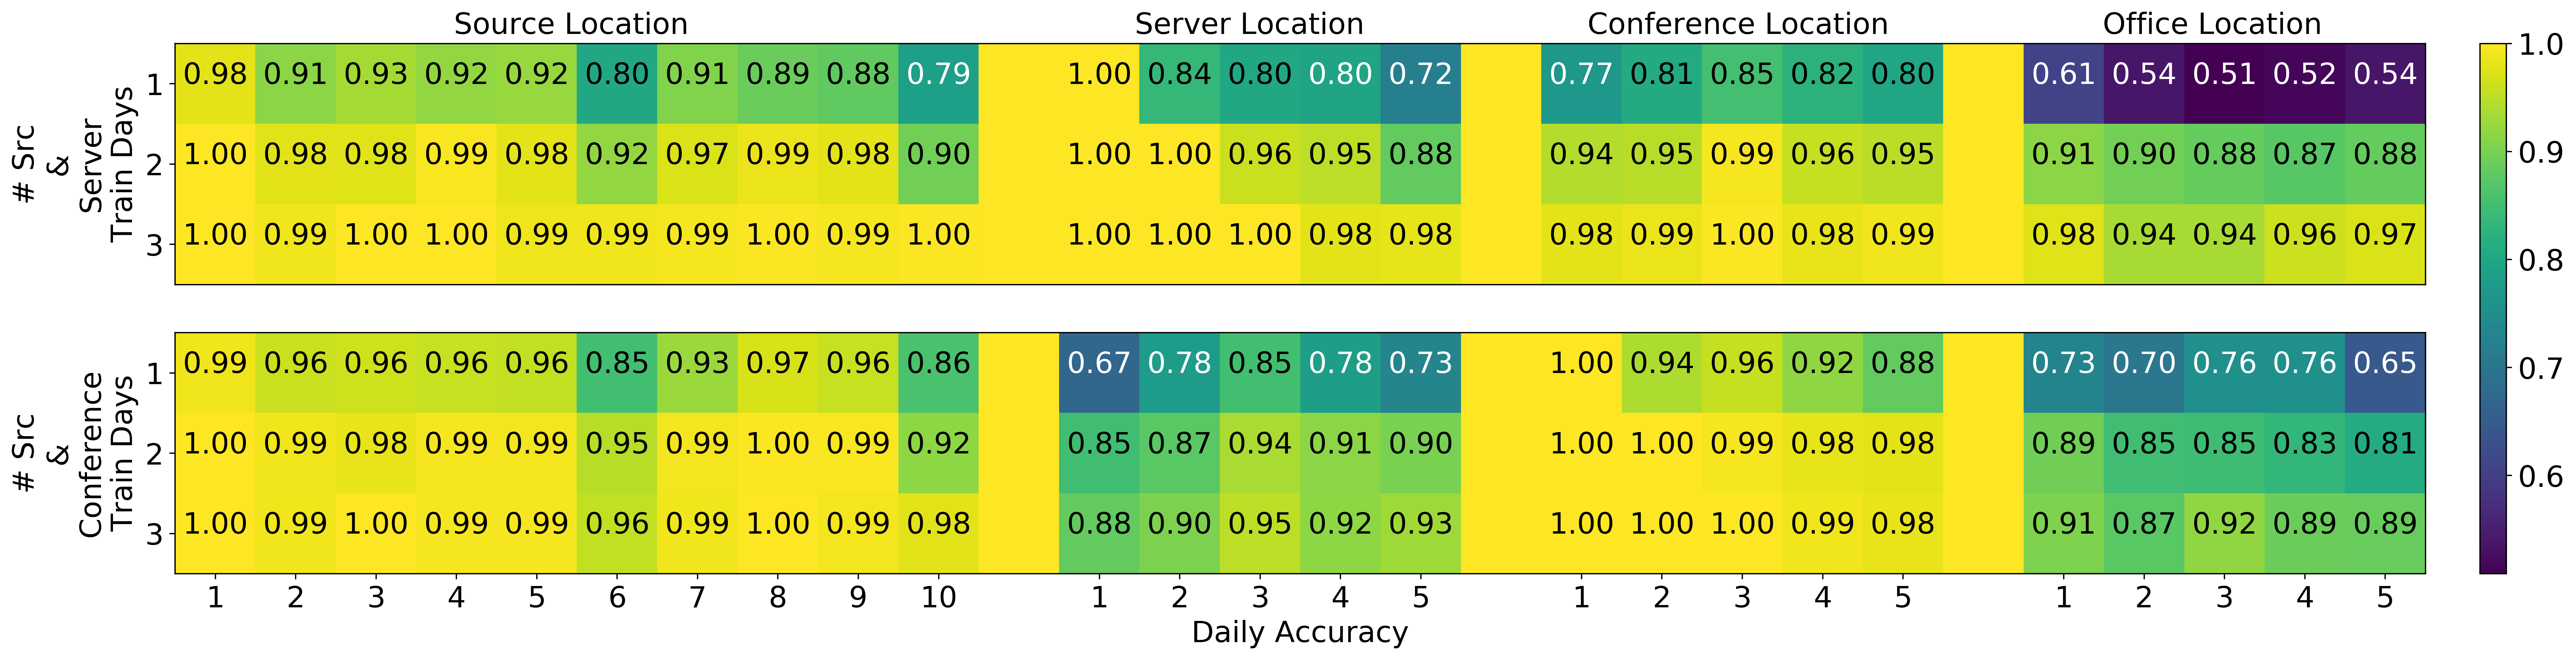
\includegraphics[width=\linewidth]{figures_supp/Exp5.png} 
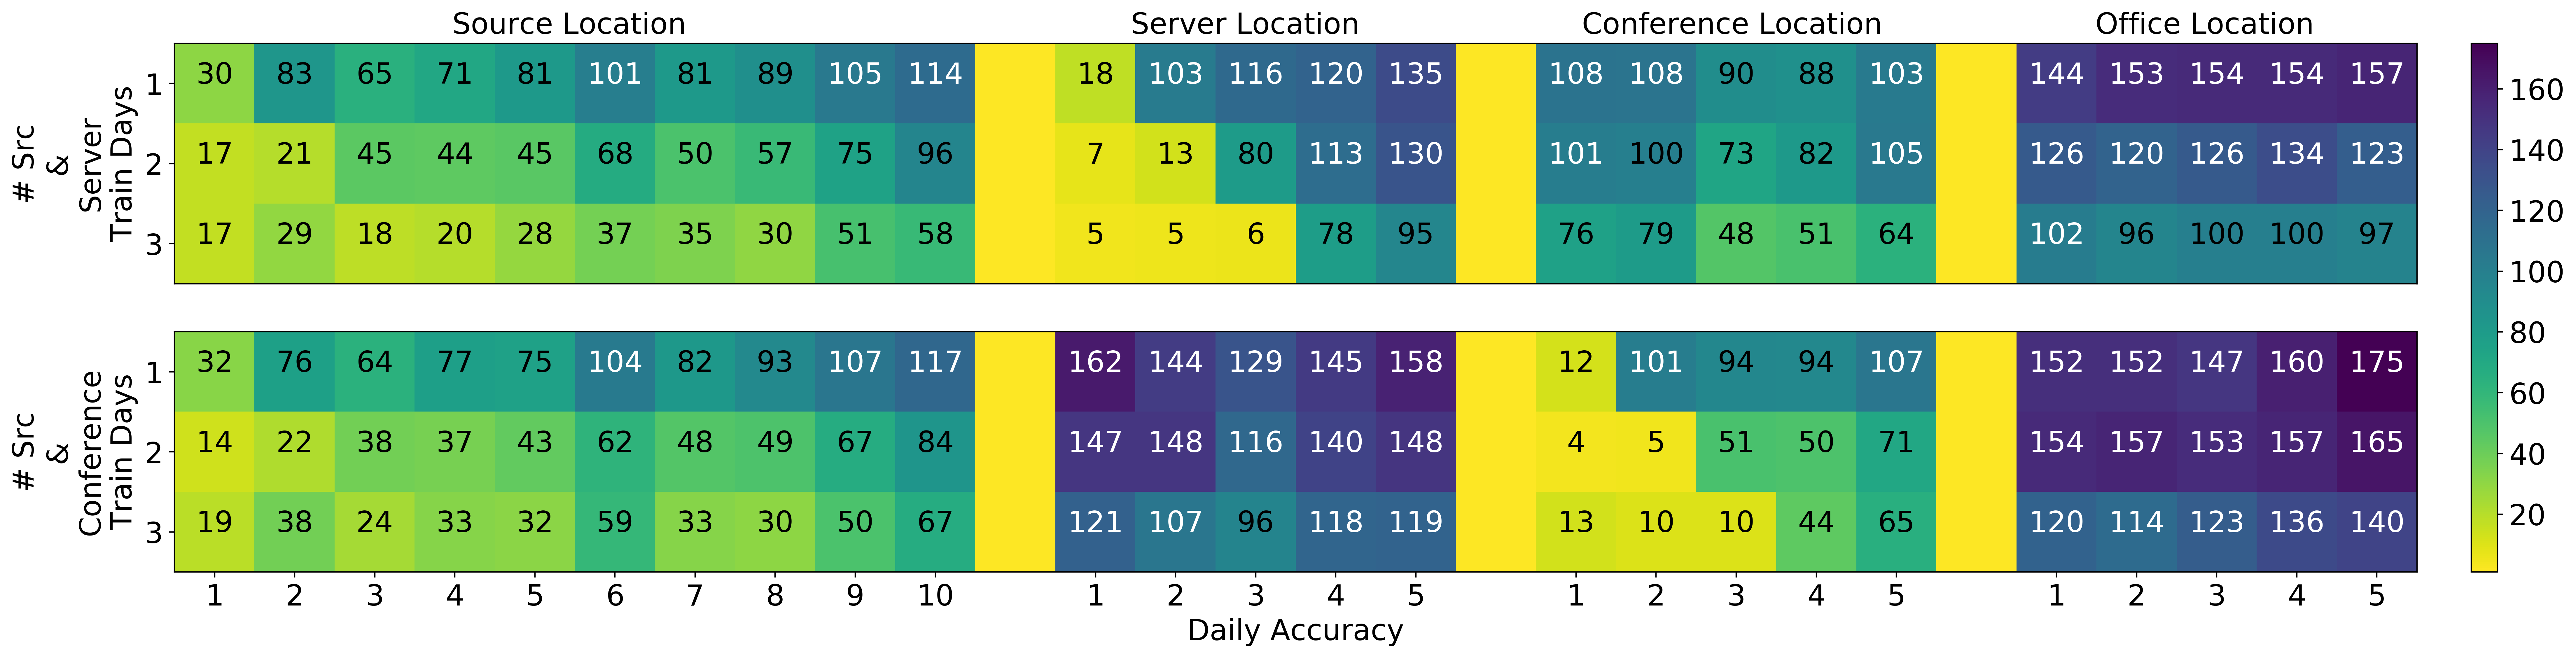
\includegraphics[width=\linewidth]{figures_supp/Exp5-metric.png} 
\caption{(Top) Results obtained from training on the source and server data for a varying number of days. (Bottom) Results obtained from training on the source and conference data for a varying number of days. Data from office location is for testing only}
\label{srctrgsep}
\end{figure}

\section{Metric Learning Based Shift and Malignancy Detection Algorithm}

We utilize Algorithm \ref{thresh} to compute thresholds used for detecting outliers. In our experiments, L2 distance was used along with a margin $m$ of 10. Upon computing class thresholds $Threshold$ and trained model $M$, any new data samples that were observed, were subject to class-wise thresholding $DistanceMetric$ between the known class centers $C^{Train}$ and the generated embedding for the new data point.   

\begin{algorithm}
    \caption{Algorithm to Compute Class-Wise Thresholds} 
    \hspace*{\algorithmicindent} \textbf{Input:} Training data $X_{Train}$, validation data $X_{Val}$, number of classes $n$, $DistanceMetric$ (L2 or cosine distance), hyperparameter safety margin $m$. \\
    \hspace*{\algorithmicindent} \textbf{Output:} Class-wise threshold $\{Threshold_j|j=1, 2, ..., n\}$, $M$, $C^{Train}$ \\

    \begin{algorithmic}[1]
        \State Train model $M$ on $X_{Train}$ with metric learning 
        \State Generate class-wise embeddings $\{C_j^{Train}|j=1, 2, ..., n\}$ from $X_{Train}$ and $M$
        \State Generate class-wise embeddings $\{C_j^{Val}|j=1, 2, ..., n\}$ from $X_{Val}$ and $M$
        \State Compute $\{Threshold_j|j=1, 2, ..., n\}$ = $DistanceMetric$ ($C_j^{Val}-C_j^{Train}|j=1, 2, ..., n$) + $m$
    \end{algorithmic} 
    \label{thresh}
\end{algorithm}

\section{GRL, GAN and Student-Teacher Methods for Unsupervised Domain Adaptation}

We addressed unsupervised domain adaptation using a GAN based approach. However, we also tried a few other methods. The most notable of which were, based on GRL and Student-Teacher(ST) based methods. We report the accuracies obtained from each method in Table~\ref{udatab}. These models were trained using three days of labeled source location data and three days of unlabeled server location data. Apart from the three methods mentioned above, we also tried introducing several other methods. Specifically, in combination with the model with GRL and AMCA loss, we tried each of the methods in \cite{zhang2017mixup, yun2019cutmix, goodfellow2014explaining, lee2013pseudo, pei2018multi, hosseini2018augmented} including mixup/cutmix regularization, adversarial training, pseudo-labels, multi-adversarial and cyclic adversarial domain adaptations. However, none of these methods amounted to any significant results. We are not sure if these methods failed as a consequence of being used along with metric learning or because the data are in the format of spectrograms. We leave investigations into the matter for our future work.  

\begin{table}[ht]
\caption{Model Accuracies (\%). (GRL) The model trained with GRL based UDA. (GAN) The model trained with GAN based UDA. (ST) The model trained with student-teacher based UDA}
\begin{center}
\begin{tabular}{ccccc} 
\hline
  & Source-Temporal & Server-Test & Conference-Test  & Office-Test \\
\hline
 GRL & 99.37 & 97.80 & 99.40 & 94.96 \\ 
\hline
 GAN & 99.61 & 98.70 & 99.70 & 97.47 \\ 
\hline
 ST & 97.77 & 86.99 & 95.50 & 85.07 \\ 
\hline
\label{udatab}
\end{tabular}
\end{center}
\end{table}

\bibliography{bibliography}

\end{document}